%&pdflatex
\documentclass{elsarticle}

\usepackage{array}
\usepackage{amsmath,amssymb,amsfonts,amsthm}
\usepackage{mathtools}
\usepackage{algorithm, algorithmic}
\usepackage{graphicx}
\usepackage{subfigure}
\usepackage{color}
\usepackage{undertilde}
\usepackage[colorlinks = true, filecolor = red, urlcolor = blue, linkcolor = black]{hyperref}

\setlength\textwidth{6in}
\setlength\textheight{8in}
\setlength\oddsidemargin{0.25in} % LaTeX adds a default 1in to this!
\setlength\evensidemargin{0.25in}
\setlength\topmargin{-0.0in} % LaTeX adds a default 1in to this!
\setlength\headsep{0in}
\setlength\headheight{0in}
\setlength\footskip{1in}

\renewcommand{\topfraction}{0.85}
\renewcommand{\textfraction}{0.1}
\renewcommand{\floatpagefraction}{0.75}

\newcommand{\vect}[1]{\ensuremath\boldsymbol{#1}}
\newcommand{\tensor}[1]{\underline{\vect{#1}}}
\newcommand{\del}{\triangle}
\newcommand{\grad}{\nabla}
\newcommand{\curl}{\grad \times}
\renewcommand{\div}{\grad \cdot}
\newcommand{\ip}[1]{\left\langle #1 \right\rangle}
\newcommand{\eip}[1]{a\left( #1 \right)}
\newcommand{\pd}[2]{\frac{\partial#1}{\partial#2}}
\newcommand{\pdd}[2]{\frac{\partial^2#1}{\partial#2^2}}

\newcommand{\Reyn}{\rm Re}

\newcommand{\bs}[1]{\boldsymbol{#1}}
\DeclareMathOperator{\diag}{diag}

\newcommand{\equaldef}{\stackrel{\mathrm{def}}{=}}

\newcommand{\tablab}[1]{\label{tab:#1}}
\newcommand{\tabref}[1]{Table~\ref{tab:#1}}

\newtheorem{remark}{Remark}

\newcommand{\theolab}[1]{\label{theo:#1}}
\newcommand{\theoref}[1]{\ref{theo:#1}}
\newcommand{\eqnlab}[1]{\label{eq:#1}}
\newcommand{\eqnref}[1]{\eqref{eq:#1}}
\newcommand{\seclab}[1]{\label{sec:#1}}
\newcommand{\secref}[1]{\ref{sec:#1}}
\newcommand{\lemlab}[1]{\label{lem:#1}}
\newcommand{\lemref}[1]{\ref{lem:#1}}

\newcommand{\mb}[1]{\mathbf{#1}}
\newcommand{\mbb}[1]{\mathbb{#1}}
\newcommand{\mc}[1]{\mathcal{#1}}
\newcommand{\nor}[1]{\left\| #1 \right\|}
\newcommand{\snor}[1]{\left| #1 \right|}
\newcommand{\LRp}[1]{\left( #1 \right)}
\newcommand{\LRs}[1]{\left[ #1 \right]}
\newcommand{\LRa}[1]{\left\langle #1 \right\rangle}
\newcommand{\LRc}[1]{\left\{ #1 \right\}}
\newcommand{\LRb}[1]{\left| #1 \right|}

\newcommand{\Grad} {\ensuremath{\nabla}}
\newcommand{\Div} {\ensuremath{\nabla\cdot}}
\newcommand{\Nel} {\ensuremath{{N^\text{el}}}}
\newcommand{\jump}[1] {\ensuremath{\LRs{\![#1]\!}}}
\newcommand{\uh}{\widehat{u}}
\newcommand{\fnh}{\widehat{f}_n}
\renewcommand{\L}{L^2\LRp{\Omega}}
\newcommand{\pO}{\partial\Omega}
\newcommand{\Gh}{\Gamma_h}
\newcommand{\Gm}{\Gamma_{-}}
\newcommand{\Gp}{\Gamma_{+}}
\newcommand{\Go}{\Gamma_0}
\newcommand{\Oh}{\Omega_h}

\newcommand{\eval}[2][\right]{\relax
  \ifx#1\right\relax \left.\fi#2#1\rvert}

\def\etal{{\it et al.~}}


\def\arr#1#2#3#4{\left[
\begin{array}{cc}
#1 & #2\\
#3 & #4\\
\end{array}
\right]}
\def\vecttwo#1#2{\left[
\begin{array}{c}
#1\\
#2\\
\end{array}
\right]}
\def\vectthree#1#2#3{\left[
\begin{array}{c}
#1\\
#2\\
#3\\
\end{array}
\right]}
\def\vectfour#1#2#3#4{\left[
\begin{array}{c}
#1\\
#2\\
#3\\
#4\\
\end{array}
\right]}
\date{}

\newtheorem{proposition}{Proposition}
\newtheorem{corollary}{Corollary}
\newtheorem{theorem}{Theorem}
\newtheorem{lemma}{Lemma}

\newcommand{\G} {\Gamma}
\newcommand{\Gin} {\Gamma_{in}}
\newcommand{\Gout} {\Gamma_{out}}

%%%%%%%%%%%%%%% End def of new commands %%%%%%%%%%%%%%%%%%%
%%%%%%%%%%%%%%% Start of thesis %%%%%%%%%%%%%%%%%%%

\begin{document}
\begin{frontmatter}

\author{Jesse Chan\corref{cor1}}
\ead{jchan@ices.utexas.edu}
\cortext[cor1]{Principal Corresponding Author, Institute for Computational Engineering and Sciences, The University of Texas at Austin}
\cortext[affil]{Institute for Computational Engineering and Sciences, The University of Texas at Austin}
\author{Leszek Demkowicz\corref{affil}}
\ead{leszek@ices.utexas.edu}
\author{Robert Moser\corref{affil}}
\ead{rmoser@ices.utexas.edu}

\title{A DPG method for steady viscous compressible flow}

\begin{abstract}
The Discontinuous Petrov-Galerkin (DPG) method is a class of novel higher order adaptive finite element methods derived from the minimization of the residual of the variational problem \cite{DPG2}, and has been shown to deliver a method for convection-diffusion that is provably robust in the diffusion parameter \cite{DPGrobustness,DPGrobustness2}.  In this work, the DPG method is extrapolated to nonlinear systems, and applied to several problems in fluid dynamics whose solutions exhibit boundary layers or singularities in stresses.  In particular, the effectiveness of DPG as a numerical method for compressible flow is assessed with the application of DPG to two model problems over a range of Mach numbers and laminar Reynolds numbers using automatic adaptivity for higher order elements, beginning with highly under-resolved coarse initial meshes.  
\end{abstract}

\end{frontmatter}

%\maketitle

%\tableofcontents

\section{Introduction}

Standard numerical methods tend to perform poorly across the board for the class of PDEs known as singular perturbation problems; these problems are often characterized by a parameter that may be either very small or very large.  An additional complication of singular perturbation problems is that very often, in the limiting case of the parameter blowing up or decreasing to zero, the PDE itself will change types (e.g.\ from elliptic to hyperbolic).  A canonical example of a singularly perturbed problem is the convection-diffusion equation in domain $\Omega \subset \mathbb{R}^3$,
\[
\div \left(\beta u\right) - \epsilon \Delta u = f.
\]
The equation models the steady-state distribution of the scalar quantity $u$, representing the concentration of a quantity in a given medium, taking into account both convective and diffusive effects. Vector $\beta \in \mathbb{R}^3$ specifies the direction and magnitude of convection, while the singular perturbation parameter $\epsilon$ represents the diffusivity of the medium. In the limit of an inviscid medium as $\epsilon\rightarrow 0$, the equation changes types, from elliptic to hyperbolic, and from second order to first order.

%We will illustrate the issues associated with numerical methods for this equation using one dimensional examples.  In 1D, the convection-diffusion equation is
%\begin{align*}
%\beta u'-\epsilon u'' &= f.
%\end{align*}
%For Dirichlet boundary conditions $u(0)=u_0$ and $u(1)= u_1$, the solution 
%can develop sharp boundary layers of width $\epsilon$ near the outflow boundary.
%\begin{figure}[!h]
%\centering
%\includegraphics[width=2.5in]{figs/GalerkinOscTight.png}
%\caption{Oscillations in the 1D finite element solution of the convection-diffusion equation for small diffusion \cite{GalerkinOsc}. Standard finite volume and finite difference methods exhibit similar behavior.}
%\label{fig:GalerkinOsc}
%\end{figure}
The standard finite element method applied to the convection-dominated diffusion problem can perform very poorly for the case of small $\epsilon$.\footnote{This is especially true in the presence of boundary layers in the solution \cite{roos2008robust}.}  This poor performance can be observed numerically -- as the singular perturbation parameter $\epsilon$ decreases, the finite element solution can diverge significantly from the best finite element approximation of the solution.  
%The poor performance of the finite element method for this problem is reflected in the bound on the error in the finite element solution --- under the standard Bubnov-Galerkin method with $u\in H^1(0,1)$, we have the bound given in \cite{roos2008robust}:
%\[
%\|u-u_h\|_\epsilon \leq C \inf_{w_h}\|u-w_h\|_{H^1(0,1)},
%\]
%for $\|u\|_\epsilon^2 \coloneqq \|u\|_{L^2}^2 + \epsilon \|u'\|_{L^2}^2$, with $C$ independent of $\epsilon$. An alternative formulation of the above bound is 
%\[
%\|u-u_h\|_{H^1(0,1)} \leq C(\epsilon) \inf_{w_h}\|u-w_h\|_{H^1(0,1)},
%\]
%where $C(\epsilon)$ grows as $\epsilon\rightarrow 0$. The dependence of the constant $C$ on $\epsilon$ is what we refer to as a \textit{loss of robustness} --- as the singular perturbation parameter $\epsilon$ decreases, our finite element error is bounded more and more loosely by the best approximation error.  As a consequence, the finite element solution can diverge significantly from the best finite element approximation of the solution for very small values of $\epsilon$.  
For example, it is well known that, on a fixed coarse mesh and for small values of $\epsilon$ (or a large Peclet number, the ratio $h/\epsilon$), the Galerkin approximation of the solution to the convection-diffusion equation with a boundary layer develops spurious oscillations everywhere in the domain, even where the best approximation error is small.  These oscillations grow in magnitude as $\epsilon \rightarrow 0$, eventually polluting the entire solution.\footnote{For nonlinear shock problems, the solution often exhibits sharp gradients or discontinuities, around which the solution would develop spurious Gibbs-type oscillations. These are a result of underresolution of the solution, and are separate from the oscillations resulting from a lack of robustness.}  

Traditionally, instability/loss of robustness in finite element methods has been dealt with using residual-based stabilization techniques.  Given some variational form, the problem is modified by adding to the bilinear form the strong form of the residual, weighted by a test function and scaled by a stabilization constant $\tau$.  The most well-known example of this technique is the streamline-upwind Petrov-Galerkin (SUPG) method, which is a stabilized FE method for solving the convection-diffusion equation using piecewise linear continuous finite elements \cite{SUPG}.  SUPG stabilization not only removes the spurious oscillations from the finite element solution of the convection-diffusion equation, but delivers the best finite element approximation in the $H^1$ norm in 1D.  

From the perspective of the compressible Navier-Stokes equations, this loss of robustness is doubly problematic.  Not only will any nonlinear solution suffer from similar unstable oscillations, but nonlinear solvers themselves may fail to yield a solution due to such instabilities.  A nonlinear solution is almost always computed by solving a series of linear problems whose solutions will converge to the nonlinear solution under appropriate assumptions, and the presence of such oscillations in each linear problem can cause the solution convergence to slow significantly or even diverge.  Artificial viscosity and shock capturing methods have been used to suppress such oscillations and regularize the problem.  While these methods will usually yield smooth and qualitatively resolved solutions, these methods are often overly diffusive, yielding results which are poor approximations of the true solution \cite{Gresho1981223}, though modern artificial viscosity and shock capturing schemes have improved greatly in recent years \cite{Barter,Guermond20114248}.  We have taken an alternative approach in this work, avoiding artificial diffusion and shock capturing for the moment.  

Our aim is to develop a stable, higher order scheme for the steady compressible laminar Navier-Stokes equations in transonic/supersonic regimes that is automatically adaptive beginning with very coarse meshes.  This requires that both the method and the refinement scheme to perform adequately on coarse meshes with high Peclet numbers -- in other words, that the adaptive method is robust in the diffusion parameter.  We construct such a method in this paper as follows: we begin by deriving the DPG method for linear problems, then constructing a DPG method for the scalar convection-diffusion equation that is robust for very small viscosities.  Unlike common adaptive methods in computational fluid dynamics, which often refine based on physical features (such as high gradients in the solution), adaptivity under this method is driven by the minimization of a residual, which measures error accurately even for highly underresolved meshes.  The DPG method for scalar convection-diffusion is then extrapolated to systems of nonlinear equations, and applied to the compressible Navier-Stokes equations.  Numerical experiments are given, demonstrating the robustness of the method and the effectiveness of automatic adaptivity for two model problems in viscous compressible flow. 


The Discontinuous Petrov-Galerkin (DPG) method of Demkowicz and Gopalakrishnan was first formulated in \cite{DPG1} as a scheme for the pure convection problem. The method demonstrated promise --- in particular, the method was able to achieve optimal convergence rates for the Peterson problem where standard DG methods were suboptimal. A breakthrough came in \cite{DPG2}, where the concept of locally-computable optimal test functions led to the development of the DPG method in its current form. Soon after, the DPG method was successfully applied to solve the convection-diffusion problem in the small-diffusion limit with $\epsilon = 1e-7$ \cite{DPG2,DPG3}. 

Historically, the name DPG was given by Bottasso, Micheletti, Sacco and Causin to their method for elliptic problems in \cite{BottassoMichelettiSacco02}. The method was then extended to other problems, including convection-diffusion, in \cite{BottassoMichelettiSacco05,CausinSacco05,CausinSaccoBottasso05}. The key point in the method of Bottasso et al.\ was their method of hybridization of fluxes. Whereas HDG methods identify an additional flux unknown on the boundary, the numerical flux coupling neighboring elements together is still typically computed in part by using contributions from interior degrees of freedom on neighboring elements. In the DPG formulation, all numerical fluxes are declared to be independent unknowns, leaving the interior field degrees of freedom completely uncoupled from element to element. This formulation is often referred to as the \emph{ultra-weak} variational formulation. 

Since its inception, the DPG method has been applied to a wide range of problems with great success, including elasticity \cite{DPGElasLocking}, thin body shell problems \cite{DPGElas}, the cloaking problem in electromagnetics \cite{DPGcloak}, both Helmholtz and elastic wave propagation problems \cite{DPG4}, and recently, the linear Stokes equation \cite{stokesDPG}. DPG has also been shown to be a generalization of several successful finite element methods --- comparisons between DPG and standard DG methods can be found in \cite{DPG1}, and more recently, several existing DG methods have been shown to be derivable using the DPG framework \cite{Bui-ThanhDemkowiczGhattas11a,DGDPG}. 

Detailed analysis of the energy setting and well-posedness of DPG has been done for the Poisson and convection-diffusion equations in \cite{analysisDPG}. The well-posedness of DPG has also recently been extended to the large class of Friedrichs systems in \cite{Bui-ThanhDemkowiczGhattas11b}. Significant efforts have also been made in demonstrating the robustness of the DPG method for singular perturbation problems, both in wave propagation \cite{DPG4,DPGwave} and convection-diffusion problems \cite{DPGrobustness, DPGrobustness2}. 

\subsection{Optimal Petrov-Galerkin methods}

\seclab{optimalTest} Petrov-Galerkin methods, in which the test space differs from the trial space, have been explored for over 30 years, beginning with the approximate symmetrization method of Barrett and
Morton~\cite{BARRETT01101981}. The idea was continued with the SUPG method of Hughes, and the characteristic Petrov-Galerkin approach of Demkowicz and Oden~\cite{Demkowicz1986188}, which introduced the
idea of tailoring the test space to change the norm in which a finite element method would converge.

The idea of optimal test functions was introduced by Demkowicz and Gopalakrishnan in \cite{DPG2}.  Conceptually, these optimal test functions are the natural result of the minimization of a residual corresponding to the operator form of a variational equation. The connection between stabilization and least squares/minimum residual methods has been observed previously \cite{GLS}. However, the method in \cite{DPG2} distinguishes itself by measuring the residual of the natural \textit{operator form of the equation}, which is posed in the dual space, and measured with the dual norm, as we now discuss. 	

Throughout this work, we assume that the trial space $U$ and test space $V$ are real Hilbert spaces, and denote $U'$ and $V'$ as the respective topological dual spaces. Let $U_h \subset U$ and $V_h\subset V$ be finite dimensional subsets. We are interested in the following problem: given $l \in V'$, find $u_h \in U_h$  such that 
%\begin{equation}
%\eqnlab{variationEq}
%\left\{
%  \begin{array}{l}
%    \text{Given } l \in V', \text{ find } u_h \in U_h  \text{ such that} \\ 
%    b(u_h,v_h) = l(v_h), \quad \forall v_h\in V_h,
%  \end{array}
%  \right.
%\end{equation}
\begin{align}
b(u_h,v_h) &= l(v_h), \quad \forall v_h\in V_h, \eqnlab{variationEq}
\end{align}
where $b\LRp{\cdot,\cdot}: U \times V \to \mbb{R}$ is a continuous
bilinear form.  $U$ is chosen to be some trial space of approximating functions, but $V_h$ is as of yet unspecified. Throughout this work, we suppose the variational problem \eqnref{variationEq} to be well-posed. 

We can identify a unique operator $B:U\rightarrow V'$ such that
\[
\langle Bu,v\rangle_V \coloneqq b(u,v), \quad u\in U, v\in V
\]
with $\LRa{\cdot, \cdot}_V$ denoting the duality pairing between $V'$ and $V$, to obtain the operator form of the continuous variational problem
\begin{equation}
\eqnlab{dualEq}
Bu = l \quad \text{in } V'.
\end{equation}
In other words, we can represent the continuous form of our variational equation
\eqnref{variationEq} equivalently as the operator equation \eqnref{dualEq} with values in the
dual space $V'$.  This motivates us to consider the conditions under which the solution to \eqnref{variationEq} is the solution to the minimum residual problem in $V'$ 
\[
u_h = \underset{u_h\in U_h}{\arg\min}\, J(u_h),
\]
where $J(w)$ is defined for $w\in U$ as 
\[
J(w) = \frac{1}{2}\|Bw-l\|_{V'}^2 \coloneqq\frac{1}{2} \sup_{v\in V\setminus\{0\}} \frac{| b(w,v)-l(v)|^2}{\nor{v}_V^2}.
\]
For convenience in writing, we will abuse the notation $\sup_{v \in V}$ to denote $\sup_{v\in V\setminus\{0\}}$ for the remainder of this work.

Let us define $R_V: V \to V'$ as the Riesz map, which identifies
elements of $V$ with elements of $V'$ by 
\[
\langle R_V v,\delta
v\rangle_V \coloneqq(v, \delta v)_V, \quad \forall \delta v \in V.
\]
Here, $(\cdot, \cdot)_V$ denotes the
inner product in $V$. As $R_V$ and its inverse, $R_V^{-1}$, are both
isometries, e.g.\ $\|f\|_{V'} = \|R_V^{-1} f\|_V, \forall f \in V'$, we
have
\begin{equation}
\eqnlab{minimization}
\min_{u_h\in U_h} J(u_h) = \frac{1}{2}\left\|Bu_h-l\right\|_{V'}^2 =  \frac{1}{2}\left\|R_V^{-1}(Bu_h-l)\right\|_V^2.
\end{equation}
The first order optimality condition for \eqnref{minimization} requires
the G\^ateaux derivative to be zero in all directions $\delta u \in U_h$, i.e.,
\begin{align*}
\left(R_V^{-1}(Bu_h-l),R_V^{-1}B\delta u\right)_V = 0, \quad \forall \delta u \in U. 
\end{align*}
We define, for a given $\delta u \in U$, the corresponding {\em optimal test function} $v_{\delta u}$
\begin{equation}
\eqnlab{optv}
v_{\delta u} \coloneqq R_V^{-1}B\delta u \quad  \text{in } V.
\end{equation} 
The optimality condition then becomes
\[
 \langle Bu_h-l, v_{\delta u}\rangle_V = 0, \quad \forall \delta u \in U
\]
which is exactly the standard variational equation in
 \eqnref{variationEq} with $v_{\delta u}$ as the test functions. We can define the optimal test space $V_{\rm opt} \coloneqq \{v_{\delta u} \text{ s.t. } \delta u\in U\}$. Thus, the solution of the variational problem \eqnref{variationEq} with test space $V_h = V_{\rm opt}$ minimizes the residual in the dual norm $\nor{Bu_h-l}_{V'}$. This is the key idea behind the concept of optimal test functions. 

Since $U_h \subset U$ is spanned by a finite number of basis functions $\LRc{\varphi_i}_{i=1}^N$, \eqnref{optv} allows us to compute (for each basis function) a corresponding optimal test function $v_{\varphi_i}$. The collection $\LRc{v_{\varphi_i}}_{i = 1}^N$ of optimal test functions then forms a basis for the optimal test space.  In order to express optimal test functions defined in \eqnref{optv} in a more familiar form, we take  $\delta u = \varphi$, a generic basis function in $U_h$, and rewrite \eqnref{optv} as
\[
R_Vv_{\varphi} = B\varphi, \quad \text{in } V',
\]
which is, by definition, equivalent to
\[
\LRp{v_\varphi,\delta v}_V = \LRa{R_Vv_\varphi,\delta v}_{V}=
\LRa{B\varphi, \delta v}_V = b\LRp{\varphi,\delta v}, \quad
\forall \delta v \in V.
\]
%% Now, let us define the \textit{trial-to-test} operator $T =
%% R_V^{-1}B$, which, by \eqnref{optv}, maps a trial function $\delta u$
%% to its corresponding \textit{optimal} test function $v = T\delta u$.
%% On the other hand,
As a result, optimal test functions can be determined by solving the auxiliary
variational problem
\begin{equation}
\eqnlab{optvVar}
\left(v_\varphi,\delta v\right)_V = b(\varphi,\delta v), \quad \forall
\delta v \in V.
\end{equation}
However, in general, for standard $H^1$ and $H({\rm div})$-conforming finite element methods, test functions are continuous over the entire domain, and hence solving variational problem \eqnref{optvVar} for each optimal test function requires a global operation over the entire mesh, rendering the method impractical. A breakthrough came through the development of
discontinous Galerkin (DG) methods, for which basis functions are
discontinuous over elements. In particular, the use of discontinuous
test functions $\delta v$ reduces the problem of determining global 
optimal test functions
in \eqnref{optvVar} to local problems that can be solved in an
element-by-element fashion.

We note that solving \eqnref{optvVar} on each element exactly is
infeasible since it amounts to inverting the Riesz map $R_V$ exactly.
Instead, optimal test functions are approximated using the standard
Bubnov-Galerkin method on an ``enriched" subspace $\tilde{V} \subset
V$ such that $\dim(\tilde{V}) > \dim(U_h)$ elementwise \cite{DPG1, DPG2}. In this
document, we assume the error in approximating the optimal test functions
is negligible, and refer to the work in \cite{practicalDPG} for
estimating the effects of approximation error on the performance of DPG.

It is now well known that the DPG method
delivers the best approximation error in the ``energy norm" --- that is
\cite{Bui-ThanhDemkowiczGhattas11a, DPG2,DPG4} 
\begin{equation}
\eqnlab{optimalError}
\nor{u-u_h}_{U,E} = \inf_{w\in U_h} \nor{u-w}_{U,E},
\end{equation}
where the energy norm $\|\cdot \|_{U,E}$ is defined for a function $\varphi \in U$ as
\begin{equation}
\eqnlab{energyNorm} \|\varphi\|_{U,E} \coloneqq \sup_{v\in V}
\frac{b(\varphi,v)}{\|v\|_V} = \sup_{\nor{v}_V = 1} b(\varphi,v) =
\sup_{\nor{v}_V = 1} \LRa{B\varphi,v}_V = \nor{B\varphi}_{V'} =
\nor{v_\varphi}_V,
\end{equation}
where the last equality holds due to the isometry of the Riesz map
$R_V$ (or directly from \eqnref{optvVar} by taking the supremum). An
additional consequence of adopting such an energy norm is that,
without knowing the exact solution, the energy error $\|u-u_h\|_{U,E}$ can
be determined by computing $\|v_{u-u_h}\|_V$ from the following
identity
\[
\left(v_{u-u_h},\delta v\right)_V = b(u-u_h,\delta v) = l\LRp{\delta
v} - b(u_h,\delta v).
\]
This is simply a consequence of the minimum-residual nature of DPG; the energy error is simply the norm of the  residual in $V'$. 

Practically speaking, this implies that the DPG method is not only discretely stable, but delivers the \emph{best approximation in the energy norm} on any mesh. In particular, the stability and optimality of DPG apply naturally to higher order adaptive meshes, where discrete stability is often an issue. 

\subsection{Ultra-weak variational formulation}
\seclab{abstractUweak}

The naming of the discontinuous Petrov-Galerkin method refers to the fact that the method is a Petrov-Galerkin method, and that the test functions are specified to be discontinuous across element boundaries. There is no specification of the regularity of the trial space, and we stress that the idea of DPG is not inherently tied to a single variational formulation \cite{Bui-ThanhDemkowiczGhattas11a}. 

In most of the DPG literature, however, the discontinuous Petrov-Galerkin method refers to the combination of the concept of locally computable optimal test functions in Section \secref{optimalTest} with the so-called ``ultra-weak formulation" \cite{DPG1,DPG2,DPG3,DPG4,DPGElas,DBLP:journals/procedia/NiemiCC11}. Unlike the previous two sections in which we studied the general equation \eqnref{variationEq} given by abstract bilinear and linear forms, we now consider a concrete instance of \eqnref{variationEq} resulting from an ultra-weak formulation for an abstract first-order system of PDEs $Au = f$. Additionally, from this section onwards, we will refer to DPG as the pairing of the ultra-weak variational formulation with the concept of locally computable optimal test functions. 

We begin by partitioning the domain of interest $\Omega$ into $\Nel$ non-overlapping elements $K_j, j = 1,\hdots,\Nel$ such that $\Oh = \cup_{j=1}^\Nel K_j$ and $\overline{\Omega} = \overline{\Omega}_h$. Here, $h$ is defined as $h= \max_{j\in \LRc{1,\hdots,\Nel}}\text{diam}\LRp{K_j}$.  We denote the mesh ``skeleton" by $\Gh = \cup_{j=1}^\Nel \partial K_j$; the set of all faces/edges $e$, each of which comes with a normal vector ${n}_e$. The internal skeleton is then defined as $\Gamma^0_h = \Gh \setminus \partial \Omega$. If a face/edge $e \in \Gh$ is the intersection of $\partial K_i$ and $\partial K_j$, $i \ne j$, we define the following jumps:
\[
\jump{v} = \text{sgn} \LRp{{n}^-}v^- + \text{sgn} \LRp{{n}^+}v^+, \quad
\jump{\tau \cdot n} = {n}^-\cdot \tau^- + {n}^+\cdot\tau^+,
\]
where
\[
\text{sgn}\LRp{{n}^{\pm}} =
\left\{
\begin{array}{ll}
1 & \text{if } {n}^{\pm} = {n}_e \\
-1 & \text{if } {n}^\pm = -{n}_e
\end{array}
\right..
\]
For $e$ belonging to the domain boundary $\partial \Omega$, we define
\[
\jump{v} = v, \quad
\jump{\tau \cdot n} = {n}_e\cdot \tau.
\]
Note that we allow arbitrariness in assigning ``-'' and ``+'' quantities to the adjacent elements $K_i$ and $K_j$.

The ultra-weak formulation for $Au = f$ on $\Oh$, ignoring boundary
conditions for now, reads
\begin{equation}
\eqnlab{uweak}
b\left(\left(u, \widehat{u}\right),v\right) \coloneqq \langle \widehat{u}, \jump{v}
\rangle_{\Gh} - (u,A_h^*v)_{\Oh}= \LRp{f,v}_{\Oh},
\end{equation}
where we have denoted $\LRa{\cdot,\cdot}_{\Gh}$ as the duality
pairing on $\Gh$, $\LRp{\cdot,\cdot}_{\Oh}$ the $L^2$-inner
product over $\Oh$, and $A_h^*$ the formal adjoint resulting from
element-wise integration by parts.  Occasionally, for simplicity in
writing, we will ignore the subscripts in the duality pairing and
$L^2$-inner product if they are $\Gh$ and $\Oh$. Both the
inner product and formal adjoint are understood to be taken
element-wise. Using the ultra-weak formulation, the regularity
requirement on solution variable $u$ is relaxed, that is, $u$ is now
square integrable for the ultra-weak formulation \eqnref{uweak} to be
meaningful, instead of being (weakly) differentiable.  The trade-off
is that $u$ does not admit a trace on $\Gh$ even though it did
originally. Consequently, we need to introduce an additional new
``trace'' variable $\widehat{u}$ in \eqnref{uweak}, that is defined only on
$\Gh$.

The energy setting is now clear; namely,
\[
u\in L^2\LRp{\Oh} \equiv L^2(\Omega), \quad v\in V=D(A^*_h), \quad
\widehat{u}\in \gamma(D(A)),
\]
where $D(A_h^*)$ denotes the broken graph space corresponding to $A_h^*$,
and $\gamma(D(A))$ the trace space (assumed to exist) of the graph space of
operator $A$. The first discussion of the well-posedness of DPG with the ultra-weak formulation can be found in \cite{analysisDPG}, where the proof is presented for the Poisson and convection-diffusion equations. A more comprehensive discussion of the abstract setting for DPG with the ultra-weak formulation using the graph space, as well as a more general proof of well-posedness, can be consulted in \cite{Bui-ThanhDemkowiczGhattas11b}. 

\subsection{Choices of test and trial norms}
\seclab{energyPair}

A clear property of the energy norm defined by \eqnref{energyNorm} is that the trial norm $\nor{\cdot}_{U,E}$ is induced by a given test norm. However, the reverse relationship holds as well; for any trial norm, the test norm that induces such a norm is recoverable through duality. We have a result, proved in \cite{Bui-ThanhDemkowiczGhattas11a}: assuming, for simplicity, that the bilinear form $b(u,v)$ is definite, given any norm $\nor{\cdot}_{U}$ on the trial space $U$, for $\varphi \in U$, we can represent $\nor{\varphi}_{U}$ via
\[
\nor{\varphi}_{U} = \sup_{v \in V}\frac{b\LRp{w,v}}{\nor{v}_{V,U}}.
\]
where $\nor{v}_{V,U}$ is defined through
\[
\nor{v}_{V,U} = \sup_{w \in U}\frac{b\LRp{w,v}}{\nor{w}_{U}}.
\]
%In other words, the norm $\nor{\cdot}_V$ in $V$ can be recovered using the energy norm $\nor{\cdot}_{U,E}$ in $U$, and vice versa. 

In particular, given two arbitrary norms $\nor{\cdot}_{U,1}$ and $\nor{\cdot}_{U,2}$ in $U$
such that $\nor{\cdot}_{U,1} \le c \nor{\cdot}_{U,2}$ for some constant
$c$, they generate two norms $\nor{\cdot}_{V,U,1}$ and
$\nor{\cdot}_{V,U,2}$ in $V$ defined by
\[
\nor{v}_{V,U,1} \coloneqq \sup_{w \in U}\frac{b\LRp{w,v}}{\nor{w}_{U,1}}, \quad
\text{and }\nor{v}_{V,U,2} \coloneqq \sup_{w \in U}\frac{b\LRp{w,v}}{\nor{w}_{U,2}},
\]
such that $\nor{\cdot}_{V,U,1}$ and $\nor{\cdot}_{V,U,2}$ induce
$\nor{\cdot}_{U,1}$ and $\nor{\cdot}_{U,2}$ as energy
norms in $U$, respectively. That is,
\[
\|\varphi\|_{U,1} = \sup_{v\in V}
\frac{b(\varphi,v)}{\|v\|_{V,U,1}}, \quad \text{and }\|\varphi\|_{U,2} = \sup_{v\in V}
\frac{b(\varphi,v)}{\|v\|_{V,U,2}}.
\]

A question that remains to be addressed is to establish the relationship
between $\nor{\cdot}_{V,U,1}$ and $\nor{\cdot}_{V,U,2}$, given that
$\nor{\cdot}_{U,1} \le c \nor{\cdot}_{U,2}$. But this is
straightforward since we have
\begin{align*}
 \| v \|_{V,U,2} = \sup_{u \in U} \frac{b\left(w,v\right)}{\left\|
  w \right\|_{U,2}} \le c\sup_{w \in U} \frac{b\left(w,v\right)}{\left\| w
  \right\|_{U,1}} = c\| v \|_{V,U,1}.
\end{align*}
Consequently, a stronger energy norm in $U$ will generate a weaker
norm in $V$ and vice versa. In other words, to show that an
energy norm $\nor{\cdot}_{U,1}$ is weaker than another energy norm
$\nor{\cdot}_{U,2}$ in $U$, one simply needs to show the reverse inequality on the
corresponding norms in $V$, that is, $\nor{\cdot}_{V,U,1}$ is stronger
than $\nor{\cdot}_{V,U,2}$.

From now on, unless otherwise stated, we will refer to $\nor{\cdot}_{V,U}$ as the test norm that induces a given norm $\nor{\cdot}_U$. Likewise, we will refer $\nor{\cdot}_{U,V}$ as the trial norm induced by a given test norm $\nor{\cdot}_V$. In this work, for simplicity of exposition, we shall call a pair of norms in $U$ and $V$ that induce each other as an {\em energy norm pairing}.

From the discussion above of energy norm and test norm pairings, we know that specifying either a test norm or trial norm is sufficient to define an energy pairing. We now derive and discuss two important energy norm pairings, the first of which begins by specifying the canonical norm in $U$ and inducing a test norm on $V$. The second pairing begins instead by specifying the canonical norm on $V$ under the ultra-weak formulation \eqnref{uweak} and inducing an energy norm on the trial space $U$.

We begin first with the canonical norm in $U$. Since $\uh \in \gamma\LRp{D\LRp{A}}$, the standard norm for $\uh$ is
the so-called minimum energy extension norm defined as
\begin{equation}
\eqnlab{MEnorm}
\|\widehat{u}\| = \inf_{w\in D\LRp{A},
  \left.w\right|_{\Gh}=\widehat{u}} \|w\|_{D\LRp{A}}.
\end{equation}
The canonical norm for the group variable $\LRp{u,\uh}$ is then given by
\[
\|\left(u,\widehat{u}\right)\|_U^2 = \|u\|^2_{\L} + \|\widehat{u}\|^2,
\]
Applying the Cauchy-Schwarz inequality, we arrive at
\[
b\LRp{\LRp{u,\uh},v} \le \nor{\LRp{u,\uh}}_U \nor{v}_{V,U},
\]
where
\[
\nor{v}_{V,U}^2 = \|A_h^*v\|_{\L}^2
+\left(\sup_{\widehat{u} \in \gamma\LRp{D\LRp{A}}} \frac{\LRa{ \widehat{u},
  \jump{v} }_{\Gh}}{\|\widehat{u}\|}\right)^2.
\]

On the other hand, since $v \in D\LRp{A^*_h}$, the canonical norm for
$v$ is the broken graph norm: 
\[
\nor{v}_V^2 =  \|A_h^*v\|_{\L}^2 + \nor{v}_{\L}^2.
\]
Using the Cauchy-Schwarz inequality again, we obtain
\[
b\LRp{\LRp{u,\uh},v} \le \nor{\LRp{u,\uh}}_{U,V} \nor{v}_{V},
\]
where
\begin{equation}
\eqnlab{inducedQuasi}
\nor{\LRp{u,\uh}}_{U,V}^2 = \nor{u}_{\L}^2
+\sup_{v \in D\LRp{A_h^*}} \frac{\LRa{\widehat{u},
  \jump{v}}_{\Gh}^2}{\|v\|_V^2},
\end{equation}

Using the framework developed in \cite{Bui-ThanhDemkowiczGhattas11a},
one can show that both pairs $\LRp{\nor{\LRp{u,\uh}}_U,
  \nor{v}_{V,U}}$ and $\LRp{\nor{\LRp{u,\uh}}_{U,V}, \nor{v}_{V}}$ are
energy norm pairings in the sense discussed in Section
\secref{energyPair}. That is, the canonical norm $\nor{\LRp{u,\uh}}_U$
in $U$ induces (generates) the norm $\nor{v}_{V,U}$ in $V$, while the
canonical norm $\nor{v}_V$ in $V$ induces (generates) the energy norm
$\nor{\LRp{u,\uh}}_{U,V}$ in $U$. In the DPG literature \cite{DPG4}, $\nor{v}_{V,U}$ is known as the {\em optimal test norm},
while $\nor{v}_{V}$ is known as the {\em quasi-optimal test norm}.

\begin{figure}[!h]
\centering
\begin{tabular}{l c c}
Trial norm & & Test norm \\
\hline
$\boxed{\|u\|^2_{\L} + \|\widehat{u}\|^2}$ & $\Longrightarrow$  & $\|A_h^*v\|_{\L}^2
+\left(\sup_{\widehat{u}} \frac{\LRa{ \widehat{u},
  \jump{v} }_{\Gh}}{\|\widehat{u}\|}\right)^2$ \\
%\hline
%Quasi-optimal trial norm & & Canonical test norm \\
%\hline
$\nor{u}_{\L}^2+\sup_{v } \left(\frac{\LRa{\widehat{u},
  \jump{v}}_{\Gh}}{\|v\|_V}\right)^2$ &  $\Longleftarrow$ & $\boxed{\|A_h^*v\|_{\L}^2 + \nor{v}_{\L}^2}$
\end{tabular}
\caption{A summary of the derivation of test/trial norm pairings; we begin with the boxed norm on either the trial or test space, and induce the norm on the other space through duality. The optimal \textit{test} norm is naturally derived by beginning with the canonical norm on the trial space, while the quasi-optimal \textit{trial} norm is derived from beginning with the canonical norm on the test space.}
\end{figure}

The canonical norm $\nor{\LRp{u,\uh}}_U$ in $U$ provides a good
balance between the standard norms on the field $u$ and the flux
$\uh$ \cite{DPG4}. As a result, if the induced norm $\nor{v}_{V,U}$ (namely, the
optimal test norm) is used to compute  optimal test functions in
\eqnref{optvVar}, the finite element error in the canonical norm is the
best in the sense of \eqnref{optimalError}. 

Unfortunately, the optimal test norm is non-localizable due to the presence of the jump term $\jump{v}$.\footnote{A localizable norm can be written as $\nor{v}_{V(\Oh)} = \sum_{K\in\Oh} \nor{v}_{V(K)},$ where $\nor{v}_{V(K)}$ is a norm over $K$.} Since the jump terms couple elements together, the evaluation of the jump terms requires contributions from all the elements in the mesh. Consequently, solving for an optimal test function
amounts to inverting the Riesz map %, defined on the left sideof \eqnref{optvVar}, 
over the entire mesh $\Oh$, making the optimal test norm impractical.

On the other hand, the quasi-optimal test norm $\nor{v}_V$, namely the canonical norm in $V$, \textit{is} localizable, and hence practical. However, it's worth noting the difference between the induced energy norm $\nor{\LRp{u,\uh}}_{U,V}$ and the canonical norm in $U$; under the induced norm $\nor{\LRp{u,\uh}}_{U,V}$ there is no natural interpretation for the norm in which the error in the flux variable $\uh$ is measured. 

Using a variant of the quasi-optimal test norm, numerical results show that the DPG method appears to provide a ``pollution-free" method without phase error for the Helmholtz equation \cite{DPG4}, and analysis of the pollution-free nature of DPG is currently under investigation. Similar results have also been obtained in the context of elasticity \cite{DPGElas} and the linear Stokes equations \cite{Camellia}. On the theoretical side, the quasi-optimal test norm has been shown to yield a well-posed DPG methodology for the Poisson and convection-diffusion equations \cite{analysisDPG}. More recently, this theory has been generalized to show the well-posedness of DPG under the quasi-optimal test norm for the large class of Friedrichs' type PDEs \cite{Bui-ThanhDemkowiczGhattas11b}.  

\section{DPG for convection-diffusion}

The convection-diffusion problem can be given as a first order system: 
\begin{align*}
\div \left(\beta u - \sigma\right) &= f\\
\frac{1}{\epsilon}\sigma - \grad u &= 0,
\end{align*}
with inflow boundary conditions $\left.u\right|_{\Gamma_{\rm in}} = u_{\rm in}$, and outflow boundary conditions $\left.u\right|_{\Gamma_{\rm out}} = u_{\rm out}$.  The inflow and outflow boundaries are defined
\begin{align*}
\Gamma_{\rm in} &\coloneqq \{x\in \Gamma; \beta_n(x) \leq 0\}, \quad {\rm (inflow)}\\ 
\Gamma_{\rm out} &\coloneqq \{x\in \Gamma; \beta_n(x) > 0\}, \quad {\rm (outflow)}
%\Gamma_{0} &\coloneqq \{x\in \Gamma; \beta_n(x) = 0\},
\end{align*}
On domain $\Omega$, with mesh $\Oh$ and mesh skeleton $\Gh$, the ultra-weak variational formulation for convection-diffusion is
\begin{align*}
b\left(\left(u,\sigma, \widehat{u}, \widehat{f}_n\right),\left( v, \tau \right)\right) &= 
\left(u,\div \tau - \beta \cdot \grad v\right)_{\Oh} + \left(\sigma, \epsilon^{-1} \tau + \grad v\right)_{\Oh} 
- \LRa{\jump{\tau\cdot n}, \widehat{u} }_{\Gh} + \LRa{ \widehat{f}_n, \jump{v} }_{\Gh}.
\end{align*}
with $v\in H^1$ and $\tau \in H({\rm div},\Oh)$. 

\subsection{Inflow boundary condition and choice of test norm}
\seclab{sec:testNormSec}

Given the above properties of DPG, we can see that the choice of test norm will determine the behavior of DPG; however, the proper choice of test norm can be unclear.  There exists a canonical graph norm for the ultra-weak variational formulation under which well-posedness can be proven for a large class of problems, and near-optimality is observed in numerical experiments \cite{DPG4, Bui-ThanhDemkowiczGhattas11b, stokesDPG}.  However, for the specific problem of convection-diffusion, the resolution of optimal test functions resulting from the graph norm prove very difficult to approximate \cite{globalLocalDPG}.  In \cite{DPGrobustness}, Demkowicz and Heuer introduced guidelines for the construction of alternative test norms based on energy estimates for the adjoint equation. We follow \cite{DPGrobustness2}, where, in addition to constructing an alternative test norm, a new inflow boundary condition is introduced in order to regularize the adjoint equation.  

Typical boundary conditions for the convection-diffusion problem enforce a Dirichlet condition on both inflow and outflow.  We adopt instead a``conserved flux'' inflow boundary condition, 
\[
\beta_nu - \epsilon\pd{u}{n} \approx u_{\rm in}.
\]
This corresponds to the imposition of a boundary condition on the conserved flux $\fnh = \beta_nu - \sigma_n$.  For small $\epsilon$ and most problems of interest, both $\pd{u}{n}$ and $\epsilon$ tend to be small, such that the above is a good approximation of $\left.u\right|_{\Gamma_{\rm in}} = u_{\rm in}$.

Under this boundary condition, the adjoint problem is regularized such that its solutions are smoother, which in turn improves the stability of the DPG method \cite{DPGrobustness2}.  We illustrate this improvement with a simple numerical experiment; Figure~\ref{fig:confusion1D} demonstrates the behavior of the DPG method under both the standard Dirichlet and the new conserved flux boundary conditions.  In both cases, the test norm used is the 1D Sobolev norm $\nor{\LRp{v,\tau}}_V\coloneqq \nor{v}_{H^1} + \nor{\tau}_{H^1}$.  The left figure shows the behavior of DPG under a Dirichlet boundary condition; degeneration of the solution is observed as $\epsilon$ decreases.  In contrast, under the new conserved flux boundary condition, as $\epsilon$ decreases, the solution converges to the $L^2$ projection of the exact solution onto our trial space.  

\begin{figure}
\centering
\subfigure[Dirichlet boundary condition $u(0) = 1$]{\includegraphics[width=2.75in]{dirichletBC.png}}
\subfigure[``Conserved flux'' boundary condition $u(0) - \epsilon u'(0) = 1$]{\includegraphics[width=2.75in]{newBC.png}}
\caption{Behavior of the 1D DPG method for convection diffusion under both standard Dirichlet and conserved flux boundary conditions.}
\label{fig:confusion1D}
\end{figure}

The test norm for convection-diffusion in multiple dimensions is defined elementwise on $K$ as
\[
\|\left(v,\tau\right)\|_{V,K}^2 = \min\left\{\frac{\epsilon}{|K|},1\right\}\|v\|^2 + \epsilon \|\grad v\|^2 + \|\beta \cdot \grad v\|^2 + \| \div \tau-\beta\cdot\grad v\|^2 + \min\left\{\frac{1}{\epsilon},\frac{1}{|K|}\right\}\|\tau\|^2.
\]
DPG under $\nor{\cdot}_V$ both delivers robust control of the $L^2$ error in the variables $u$ and $\sigma$ and minimizes approximation error in the solution of \eqnref{optvVar}.

\subsection{Anisotropic refinement}
\seclab{sec:aniso}
Isotropic adaptive mesh refinement has shown itself to be an effective way to resolve isolated solution features with large gradients, such as point singularities \cite{hp1,hp3}. However, for the resolution of phenomena such as shocks or boundary layers, anisotropic mesh refinement can resolve solution features for a much lower cost per degree-of-freedom, due to the fact that boundary layers in $n$-dimensions are primarily phenomena supported over $n-1$ dimensions.  

As a least squares method, DPG already includes a natural error indicator with which to drive adaptive mesh refinement.  To introduce anisotropic refinements, we need to introduce an anisotropy indicator in order to detect in which direction solution features are aligned.  In general, a test norm can be expressed as the sum of normed quantities, both scalar and vector valued.  If we restrict ourselves to quadrilateral elements for the moment, a general anisotropy indicator for DPG can be constructed by evaluating the $\L$ norms of the individual components of vector valued terms in the test norm.  

Under the robust test norm derived in this chapter for the convection-dominated diffusion problem, we can define $x$ and $y$ error contributions over a single element
\begin{align*}
e_{x,K} &= \epsilon \nor{\pd{v}{x}}_{L^2(K)}^2 + \nor{\tau_x}_{L^2(K)}^2 \\
e_{y,K} &= \epsilon \nor{\pd{v}{y}}_{L^2(K)}^2 + \nor{\tau_y}_{L^2(K)}^2.
\end{align*}
We define the anisotropy indicator as the ratio $r_K = \frac{e_{x,K}}{e_{y,K}}$, and implement a simple refinement scheme following \cite{DPG3}.  Given some anisotropic threshold $\epsilon_r$, if $r_K>\epsilon_r$, then we can conclude that the error in the $x$ direction is large compared to the $y$ direction, and we anisotropically refine the element along the $x$-axis.  Likewise, if $r_K < \frac{1}{\epsilon_r}$, this implies that the opposite is true, and we refine the element anisotropically along the $y$-axis.  

%We note that it is possible to compute the discrete system without needing much additional integration.  Recall that if we let $G$ be the symmetric positive-definite Gram matrix representing the inner product $\LRp{v,\delta v}_V$ on $V_h$, we solve for degrees of freedom $c_e$ representing our error representation function $e$.  
%
%For both the graph and robust test norms, we can decompose the inner product that induces the test norm into 
%\[
%\LRp{v,\delta v}_V = \sum_i \LRp{v,\delta v}_{V,x_i} + \LRp{v,\delta v}_{V,{\rm scalar}}
%\]
%such that $\LRp{v,\delta v}_{V,x_i}$ is a seminorm containing the $i$th coordinate component of a vector-valued test term, and $\LRp{v,\delta v}_{V,{\rm scalar}}$ is simply the non-vector portions of the test norm.  For example, if we take the $H^1(\Omega)$ Sobolev norm
%\[
%\LRp{v,\delta v}_V = \LRp{v,\delta v}_{\L} + \LRp{\grad v,\grad \delta v}_{\L}
%\]
%then $\LRp{v,\delta v}_{V,x_i} = \LRp{\pd{v}{x_i},\pd{\delta v}{x_i}}_{\L}$, and $\LRp{v,\delta v}_{V,{\rm scalar}} = \LRp{v,\delta v}_{\L}$.  Each bilinear term $\LRp{v,\delta v}_{V,x_i}$ induces a symmetric positive-semidefinite matrix $G_{x_i}$, such that 
%\[
%c_e^TG_{x_i}c_e = \nor{e}^2_{V,x_i}.
%\]
%By storing $G$ as the sum of $G_{\rm scalar}$ and $G_{x_i}$, we can then cheaply compute the anisotropic error indicators once we have the degrees of freedom corresponding to our error representation function.  



\section{DPG for nonlinear problems}
\section{The viscous Burgers equation}

We will begin with the viscous Burgers' equation as an example of 

\begin{figure}[!h]
\centering
\includegraphics[scale=.5]{figs/burgers1e4.png}
\caption{Shock solution for Burgers' equation with $\epsilon = 10^{-4}$.} 
\end{figure}

\section{The compressible Navier-Stokes equations}

We briefly review the 2D compressible Navier-Stokes equations and formulate DPG for the nonlinear system. 
\begin{itemize}
\item \textbf{Conservation equations}
\begin{align*}
\div \vecttwo{\rho u_1 }{\rho u_2} &= 0\\
\div \vecttwo{\rho u_1^2+p }{\rho u_1 u_2} &= \div\left(\vec{\sigma_{i1}}\right)\\
\div \vecttwo{\rho u_1 u_2}{\rho u_2^2+p } &= \div\left(\vec{\sigma_{i2}}\right)\\
\div\vecttwo{((\rho e)+p)u_1}{((\rho e)+p)u_2} &= \div\left[\boldsymbol\sigma \boldsymbol u + \vec{q}\right],
\end{align*}
where $\boldsymbol \sigma$ is the stress tensor whose $ij$th term is $\sigma_{ij}$, and $\boldsymbol u$ is the vector $(u_1,u_2)^T$.  

\item \textbf{Newtonian fluid laws}

We represent $\boldsymbol\sigma$ using the Newtonian fluid law
\[
\sigma_{ij} = \mu(u_{i,j} + u_{j,i}) + \lambda u_{k,k} \delta_{ij}
\]
where $\mu$ is viscosity and $\lambda$ is bulk viscosity. 
%Following elasticity, a general formula for the stress tensor is 
%\[
%\sigma_{ij} = 2\mu \epsilon_{ij} + \lambda \epsilon_{kk} \delta_{ij}
%\]
We can invert the stress tensor under isotropic and plane strain assumptions to get
\[
\frac{1}{2}\left(\grad  \boldsymbol u + \grad ^T  \boldsymbol u\right) = \frac{1}{2\mu} \sigma_{ij} - \frac{\lambda}{4\mu (\mu + \lambda)} \sigma_{kk}\delta_{ij}
\]
We also have
\[
\frac{1}{2}\left(\grad  \boldsymbol u + \grad ^T  \boldsymbol u\right) = \grad  \boldsymbol u - \boldsymbol \omega
\]
where $\boldsymbol \omega$ is the antisymmetric part of the infinitesimal strain tensor:
\[
\boldsymbol \omega = \frac{1}{2}\left(\grad  \boldsymbol u - \grad ^T  \boldsymbol u\right).
\]
Thus our final form is
\begin{align*}
\grad  \boldsymbol u - \boldsymbol \omega = \frac{1}{2\mu} \boldsymbol \sigma - \frac{\lambda}{4\mu (\mu + \lambda)} { \rm tr}(\boldsymbol \sigma) \boldsymbol I.
\end{align*}
Notice that $\boldsymbol \omega$ is implicitly defined to be the antisymmetric part of $\grad u$ by taking the symmetric part of the above equation. 

We note that, though this is a standard approach in solid mechanics, it is nonstandard compared to the usual finite element and DG approaches to the viscous stresses. We adopt such an approach to better mirror our experiences with the convection-diffusion equation \cite{DPGrobustness,DPGrobustness2}. 

\item \textbf{Fourier's heat conduction law}

We assume Fourier's law 
\begin{align*}
\vec{q} &= \kappa \grad T,
\end{align*}
%where $\kappa$ is generally a function of temperature. 
We introduce here the Prandtl number here as well
\[
{\rm Pr} = \frac{\gamma c_v \mu}{\kappa}.
\]
In this case, we assume a constant Prandlt number, which implies that the heat conductivity $\kappa$ is proportional to viscosity $\mu$.

\end{itemize}

\subsection{Nondimensionalization}
To nondimensionalize our equations, we introduce nondimensional quantities for length, density, velocity, temperature, and viscosity. 
\[
\boldsymbol x^* = \frac{\boldsymbol x}{L}, \qquad \rho^* = \frac{\rho}{\rho_{\infty}}, \qquad u_1^* = \frac{u_1}{V_\infty}, \qquad u_2^* = \frac{u_2}{V_\infty}, \qquad T^* = \frac{T}{T_\infty}, \qquad \mu^* = \frac{\mu}{\mu_\infty}
\]
Pressure, internal energy, and bulk viscosity are then nondimensionalized with respect to the above variables
\[
p^* = \frac{p}{\rho_\infty V_\infty^2}, \qquad \iota^* = \frac{\iota}{V_\infty^2}, \qquad \lambda^* = \frac{\lambda}{\mu_\infty}
\]
We introduce, for convenience, the Reynolds number
\[
\Reyn = \frac{\rho_\infty V_\infty L}{\mu_\infty} 
\]
and the reference (free stream) Mach number
\[
M_\infty = \frac{V_\infty}{\sqrt{\gamma(\gamma-1)c_vT_\infty}}
\]
Note that 
\[
a = \sqrt{\frac{\gamma p_\infty}{\rho_\infty}} = \sqrt{{\gamma p_\infty}} = \sqrt{\gamma(\gamma-1)c_vT_\infty}
\]
The equations take the same form as before after nondimensionalization, so long as we define new material constants
\[
\tilde{\mu} = \frac{\mu^*}{\Reyn}, \qquad \tilde{\lambda} = \frac{\lambda^*}{\Reyn}, \qquad \tilde{c}_v = \frac{1}{\gamma(\gamma-1)M_\infty^2}, \qquad \tilde{\kappa} = \frac{\gamma\tilde{c}_v\tilde{\mu}}{\rm Pr}
\]
From here on, we drop the $^*$ superscript and assume all variables refer to their nondimensionalized quantities.

To summarize, our system of equations in the classical variables is now
\begin{align*}
\div \vecttwo{\rho u_1 }{\rho u_2} &= 0\\
\div \left(\vecttwo{\rho u_1^2+p }{\rho u_1 u_2} - \boldsymbol \sigma_{1}\right) &=0\\
\div \left(\vecttwo{\rho u_1 u_2}{\rho u_2^2+p } - \boldsymbol \sigma_{2}\right) &=0\\
\div \left(\vecttwo{((\rho e)+p)u_1}{((\rho e)+p)u_2} - \boldsymbol\sigma \mathbf{u} - \vec{q}\right) &=0\\
\frac{1}{2\mu} \boldsymbol \sigma - \frac{\lambda}{4\mu (\mu + \lambda)} { \rm tr}(\boldsymbol \sigma) \boldsymbol I &= \grad \mathbf{u} - \Reyn \, {\boldsymbol \omega}\\
\frac{1}{\kappa}\vec{q} &= \grad T
\end{align*}
We strongly enforce symmetry of the stress tensor $\boldsymbol \sigma$ by setting $\sigma_{21} = \sigma_{12}$. Additionally, we have scaled the antisymmetric tensor $\boldsymbol \omega$ by the Reynolds number to ensure that $\boldsymbol \omega = O(1)$ for all ranges of $\Reyn$.  

\subsection{Linearization}

As the equations for viscous compressible flow are nonlinear and cannot be solved exactly, we linearize the equations and adopt an iterative procedure for approximating the nonlinear solution.\footnote{We note that it is possible to linearize the strong form of the equations and then derive a linearized weak form, instead of linearizing the weak form of the nonlinear equations, which is done here.  The two formulations are equivalent; however, extraneous linearization of the fluxes is avoided using the latter approach.}  We outline the linearization of both the conservation and stress laws in this section.

\subsubsection{Conservation laws}

The Navier-Stokes conservation laws can be written as 
\begin{align*}
\div \vecttwo{\rho u_1 }{\rho u_2} &= 0\\
\div \left(\vecttwo{\rho u_1^2+p }{\rho u_1 u_2} - \boldsymbol \sigma_{1}\right) &=0\\
\div \left(\vecttwo{\rho u_1 u_2}{\rho u_2^2+p } - \boldsymbol \sigma_{2}\right) &=0\\
\div \left(\vecttwo{((\rho e)+p)u_1}{((\rho e)+p)u_2} - \boldsymbol \sigma_1 \cdot \boldsymbol u- \boldsymbol \sigma_2 \cdot \boldsymbol u - \vec{q}\right) &=0,
\end{align*}
where $\boldsymbol \sigma_1$ is the $i$th column or row of $\boldsymbol \sigma$, or more generally, if we group our Eulerian and stress variables into the vector variables $\boldsymbol U$ and $\boldsymbol \Sigma$, respectively
\[
\div (F_i(\boldsymbol U)-G_i(\boldsymbol U,\boldsymbol \Sigma) = 0, \qquad i = 1,\ldots, 4,
\]
where $F_i$and $G_i$ are given as
\begin{align*}
F_1 = \vecttwo{\rho u_1 }{\rho u_2}, \quad &G_1 = 0\\
F_2 = \vecttwo{\rho u_1^2+p }{\rho u_1 u_2},\quad &G_2 = \boldsymbol \sigma_{1}\\
F_3 = \vecttwo{\rho u_1 u_2}{\rho u_2^2+p }, \quad &G_3 = \boldsymbol \sigma_{2}\\
F_4 = \vecttwo{((\rho e)+p)u_1}{((\rho e)+p)u_2}, \quad &G_4 = \boldsymbol \sigma_1 \cdot \boldsymbol u + \boldsymbol \sigma_2 \cdot \boldsymbol u + \vec{q}
\end{align*}
The variational form restricted to a single element gives
\[
\langle \widehat{F}_i\cdot n, v\rangle - \int_K  (F(\boldsymbol U)-G_i(\boldsymbol U,\boldsymbol \Sigma)) \cdot \grad v_i = 0 , \qquad i = 1,\ldots, 4
\]
and the variational form over the entire domain is given by summing up the element-wise contributions. 

The presence of terms such as $\boldsymbol \sigma_i \cdot \boldsymbol u$ means that we will need to linearize in the stress variables $\sigma_ij$ in addition to our Eulerian quantities. Since fluxes and traces are linear functions of the unknowns, we do not need to linearize them. Instead, fluxes $\widehat{F}_{i,n}$ and traces $\widehat{u},\widehat{v},\widehat{T}$ will represent normal traces and traces of the accumulated nonlinear solution. The linearized variational formulation is thus
\begin{align*}
\langle \widehat{F}_i\cdot n, v\rangle &- \int_K  \left(F_{i,\boldsymbol U}(\boldsymbol U)\cdot \Delta \boldsymbol U -G_{i,\boldsymbol U}(\boldsymbol U, \boldsymbol \Sigma)\cdot \Delta \boldsymbol U - G_{i,\boldsymbol \Sigma}(\boldsymbol U, \boldsymbol \Sigma)\cdot \Delta \boldsymbol \Sigma \right)\cdot \grad v_i \\
&= \int_K  \left(F_i(\boldsymbol U)-G_i(\boldsymbol U)\right) \cdot \grad v_i \\
\qquad i &= 1,\ldots, 4
\end{align*}
where $F^i_{j,\boldsymbol U}$, $G^i_{j,\boldsymbol U}$, and $G^i_{j,\boldsymbol \Sigma}$ are the Eulerian and two viscous Jacobians (linearized w.r.t.\ the Eulerian/viscous variables), respectively.
%where
%\begin{align*}
%F^1_{1,\boldsymbol U} &= \{u,\rho ,0,0\} \\
%F^2_{1,\boldsymbol U} &= \{v,0,\rho ,0\} \\
%F^1_{2,\boldsymbol U} &=\left\{c_v T (\gamma -1)+u^2,2 u \rho ,0,c_v (\gamma -1) \rho \right\}\\
%F^2_{2,\boldsymbol U} &=\{u v,v \rho ,u \rho ,0\}\\
%F^1_{3,\boldsymbol U} &=\{u v,v \rho ,u \rho ,0\}\\
%F^2_{3,\boldsymbol U} &=\left\{c_v T (\gamma -1)+v^2,0,2 v \rho ,c_v (\gamma -1) \rho \right\}\\
%F^1_{4,\boldsymbol U} &=\left\{\frac{1}{2} u \left(2 c_v T (2 \gamma -1)+u^2+v^2\right),\frac{1}{2} \rho  \left(2 c_v T (2 \gamma -1)+3 u^2+v^2\right),u v \rho ,c_v u (2 \gamma -1) \rho \right\}\\
%F^2_{4,\boldsymbol U} &=\left\{\frac{1}{2} v \left(2 c_v T (2 \gamma -1)+u^2+v^2\right),u v \rho ,\frac{1}{2} \rho  \left(2c_v T (2 \gamma -1)+u^2+3 v^2\right),c_v v (2 \gamma -1) \rho \right\}
%\end{align*}
%The viscous Jacobians become (when linearized with respect to $\{\sigma_{11},\sigma_{12}, \sigma_{22}\}$)
%\begin{align*}
%G^1_{2,\boldsymbol \sigma} &= \{1,0,0\}\\
%G^2_{2,\boldsymbol \sigma} &= \{0,1,0\}\\
%G^1_{3,\boldsymbol \sigma} &= \{0,1,0\}\\
%G^2_{3,\boldsymbol \sigma} &= \{0,0,1\}\\
%G^1_{4,\boldsymbol \sigma} &= \{u_1,u_2,0\}\\
%G^2_{4,\boldsymbol \sigma} &= \{0,u_1,u_2\}
%\end{align*}
%and (when linearized with respect to the Eulerian variables)
%\begin{align*}
%G^1_{4,\boldsymbol U} &= \{0,\sigma_{11},\sigma_{12},0\}\\
%G^2_{4,\boldsymbol U} &= \{0,\sigma_{12},\sigma_{22},0\}
%\end{align*}

\subsubsection{Viscous equations}
We have two equations left to linearize - the constitutive laws defining our viscous stresses and heat flux terms. 
\begin{align*}
\frac{1}{2\mu}{\boldsymbol \sigma}- \frac{\lambda}{4\mu(\mu+\lambda)}{\rm tr}({\boldsymbol \sigma}){\boldsymbol I} + \Reyn {\boldsymbol \omega} &= 
\grad
\left[\begin{array}{c}
u_1\\
u_2
\end{array}
\right]\\
\frac{1}{\kappa}
\left[\begin{array}{c}
q_1\\
q_2
\end{array}\right] &=
\grad T
\end{align*}

We treat the first tensor equation as two vector equations by considering each column:
\begin{align*}
\frac{1}{2\mu} \vecttwo{\sigma_{11}}{\sigma_{12}} - \frac{\lambda}{4\mu(\mu+\lambda)}\vecttwo{\sigma_{11}+\sigma_{22}}{0} + \Reyn\vecttwo{0}{-\omega} - \grad u_1&= 0 \\
\frac{1}{2\mu} \vecttwo{\sigma_{12}}{\sigma_{22}} - \frac{\lambda}{4\mu(\mu+\lambda)}\vecttwo{0}{\sigma_{11}+\sigma_{22}} + \Reyn\vecttwo{\omega}{0} - \grad u_2 &= 0
\end{align*}
%These equations are linear in $\sigma_{ij}$, so the linearization is simple. 
Since all equations are linear in variables $q_1, q_2, w$ for all combinations of variables, we do not need to linearize any equations in $q_1, q_2, w$.  We do not linearize the viscosities $\mu$ and $\lambda$, but instead set them based on the power law and the solution at the previous timestep for simplicity. 

\subsection{Test norm}

%Recall the convection-diffusion problem 
%\begin{align*}
%\div \left(\beta u - \sigma\right) &= f\\
%\frac{1}{\epsilon}\sigma - \grad u &= 0.
%\end{align*}
%On domain $\Omega$, with mesh $\Oh$ and mesh skeleton $\Gh$, the DPG variational formulation is
%\begin{align*}
%b\left(\left(u,\sigma, \widehat{u}, \widehat{f}_n\right),
%\left( v, \tau \right)\right) = \left(u,\div \tau - \beta \cdot \grad
%v\right)_{\Oh} + \left(\sigma, \epsilon^{-1} \tau + \grad v\right)_{\Oh} - \LRa{
%\jump{\tau\cdot n}, \widehat{u} }_{\Gh} + \LRa{ \widehat{f}_n,
%  \jump{v} }_{\Gh}.
%\end{align*}
%with $v\in H^1$ and $\tau \in H({\rm div},\Oh)$. The test norm adopted for convection-diffusion in \cite{DPGrobustness2} is defined elementwise on $K$ as
%\[
%\|\left(v,\tau\right)\|_{V,K}^2 = \min\left\{\frac{\epsilon}{|K|},1\right\}\|v\|^2 + \epsilon \|\grad v\|^2 + \|\beta \cdot \grad v\|^2 + \| \div \tau-\beta\cdot\grad v\|^2 + \min\left\{\frac{1}{\epsilon},\frac{1}{|K|}\right\}\|\tau\|^2.
%\]
%This test norm both delivers robust control of the error in the $L^2$ variables $u$ and $\sigma$ and avoids boundary layers in the computation of local test functions. 

Recall that the test norm adopted for convection-diffusion is defined elementwise as
\[
\|\left(v,\tau\right)\|_{V,K}^2 = \min\left\{\frac{\epsilon}{|K|},1\right\}\|v\|^2 + \epsilon \|\grad v\|^2 + \|\beta \cdot \grad v\|^2 + \| \div \tau-\beta\cdot\grad v\|^2 + \min\left\{\frac{1}{\epsilon},\frac{1}{|K|}\right\}\|\tau\|^2.
\]
This test norm is extrapolated to the Navier-Stokes equations as follows: we denote the vector of $H^1$ test functions as $\boldsymbol V=\{v_1,v_2,v_3,v_4\}$, and similarly for $\boldsymbol W = \{\tau_1,\tau_2,\tau_3\}$. If $R_{\rm Euler}(\boldsymbol U,\boldsymbol \Sigma)$ and $R_{\rm visc}(\boldsymbol U,\boldsymbol \Sigma)$ are Eulerian and viscous nonlinear residuals, our formulation for the linearized Navier-Stokes equations can be written as
\begin{align*}
\div \left(A_{\rm Euler}\boldsymbol \delta U - A_{\rm visc}\boldsymbol \delta \Sigma\right) &= R_{\rm Euler}(\boldsymbol U,\boldsymbol \Sigma)\\
E_{\rm visc}\boldsymbol  \delta \Sigma - \grad \boldsymbol \delta U &= R_{\rm visc}(\boldsymbol U,\boldsymbol \Sigma)
\end{align*}
with variational formulation
\begin{align*}
\LRa{\widehat{F}_n,\boldsymbol V}_{\Gh} + \left(\boldsymbol \delta U,\div \boldsymbol W - A_{\rm Euler}^T\grad \boldsymbol  V\right) + \LRa{\widehat{\boldsymbol U},\boldsymbol W\cdot n}_{\Gh} + \left(\boldsymbol \delta \Sigma,E_{\rm visc}^T\boldsymbol W - A_{\rm visc}^T\grad \boldsymbol  V\right) &= 
\\ \LRa{R_{\rm Euler}(\boldsymbol U,\boldsymbol \Sigma),\boldsymbol V} + \LRa{R_{\rm visc}(\boldsymbol U,\boldsymbol \Sigma),\boldsymbol W}
\end{align*}
Identifying vector-valued terms in the Navier-Stokes formulation with equivalent scalar terms in the convection-diffusion equation allows us to extrapolate our test norm to systems of equations
\begin{align*}
\|\left(\boldsymbol V,\boldsymbol W\right)\|_{V, K}^2 =& \|\boldsymbol V\|^2 + \frac{1}{\Reyn} \|A_{\rm visc}^T\grad \boldsymbol V\|^2 + \|A_{\rm Euler}^T \grad \boldsymbol V\|^2 \\
& + \| \div \boldsymbol W - A_{\rm Euler}^T \grad \boldsymbol V\|^2 + \min\left\{\Reyn,\frac{1}{|K|}\right\}\|E_{\rm visc}^T\boldsymbol W\|^2.
\end{align*}
An advantage of this extrapolation approach is that the incompletely parabolic nature of the Navier-Stokes equation is taken into account; there is no diffusive term present in the mass conservation equation, and the test norm reflects that by requesting only limited regularity of $v_1$, the test function for the conservation equation.\footnote{The situation is analogous to using the full $H^1(\Oh)$ norm for the pure convection equation --- the optimal test norm $\nor{v}_V = \nor{\beta\cdot \grad v} + \nor{v}$ implies only streamline regularity, whereas taking $\nor{v}_V = \nor{\grad v} + \nor{v}$ implies stronger regularity on the test space $V$ than the graph norm. Consequently, convergence is suboptimal for DPG applied to the convection problem under the $H^1(\Oh)$ test norm.}

\subsection{Boundary conditions}

As a consequence of the ultra-weak variational formulation, our solution is linear in the flux and trace variables. Thus, the nonlinear boundary conditions can be applied directly to our fluxes $\widehat{f}_{i,n}, i = 1,\ldots,4$, and traces $\widehat{u}_1$, $\widehat{u}_2$, and $\widehat{T}$. Additionally, inflow boundary conditions are applied not directly to the trace variables $\widehat{u}_1$, $\widehat{u}_2$, and $\widehat{T}$, but to the fluxes $\widehat{f}_{i,n}$. Extrapolating from the convection-diffusion problem, this allows us to use a stronger test norm without experiencing adverse effects for smaller diffusion/higher Reynolds numbers, as described in Section~\secref{sec:testNormSec} and \cite{DPGrobustness,DPGrobustness2}.

\section{Nonlinear solver}

For our nonlinear solver, we use a pseudo-time stepping approach to iterate to a steady state solution, along with a greedy refinement scheme to eliminate spatial discretization error.  We cover briefly the details of the pseudo-timestepping method in this section.  
%Though we have not yet implemented adaptive timestepping, we are able to take large enough uniform timesteps over a coarse mesh such that convergence occurs sufficiently quickly.

\subsection{Pseudo-timestepping}

The solution of the compressible Navier-Stokes equations can be quite challenging; as mentioned previously, the direct application of a Newton algorithm often will not converge, especially for high Reynolds numbers.  Typically, a pseudo-timestepping algorithm is used in lieu of a full nonlinear Newton algorithm. The pseudo-timestep proceeds as follows: given the transient terms present in the conservation laws of compressible flow
\begin{align*}
\pd{\rho}{t} + \ldots \\
\pd{\LRp{\rho u}}{t} + \ldots \\
\pd{\LRp{\rho v}}{t} + \ldots \\
\pd{\LRp{\rho e}}{t} + \ldots,
\end{align*}
we discretize each time derivative using an implicit timestepping method.  Though second order time discretizations have been shown to be effective \cite{Demkowicz1990275, BenKirk}, we choose a first order backwards Euler discretization for simplicity.  Due to the fact that we've chosen to solve the Navier-Stokes equations under primitive variables $\rho, u, v$, and $T$, the time terms are nonlinear as well, and must be linearized.  After time discretization and linearization, we are left with a coupled system of reaction terms in the problem for our solution update at every timestep
\begin{align*}
A_{\rm time}\boldsymbol \delta U_i + \div \left(A_{\rm Euler}\boldsymbol \delta U_i - A_{\rm visc}\boldsymbol \delta \Sigma_i\right) &= R_{\rm Euler}(\boldsymbol U_i,\boldsymbol \Sigma_i) + R_{\rm time}(\boldsymbol U_{i-1},\boldsymbol U_i)\\
E_{\rm visc} \boldsymbol \Sigma_i - \grad \boldsymbol U_i &= R_{\rm visc}(\boldsymbol U_i,\boldsymbol \Sigma_i),
\end{align*}
where $R_{\rm time}(\boldsymbol U_{i-1},\boldsymbol U_i)$ is the transient residual.  Including the transient terms in our test norm as well, our final test norm is 
\begin{align*}
\|\left(\boldsymbol V,\boldsymbol W\right)\|_{V,K}^2 =& \nor{A_{\rm time}^T\boldsymbol V} + \|\boldsymbol V\|^2 + \frac{1}{\Reyn} \|A_{\rm visc}^T\grad \boldsymbol V\|^2 + \|A_{\rm Euler}^T \grad \boldsymbol V\|^2 \\
& + \| \div \boldsymbol W - A_{\rm Euler}^T \grad \boldsymbol V\|^2 + \min\left\{\Reyn,\frac{1}{|K|}\right\}\|E_{\rm visc}^T\boldsymbol W\|^2.
\end{align*}
Finally, convergence of the pseudo-timestepping method is determined by measuring the transient residual in the energy norm; in other words, we measure $\nor{e_{\rm time}}_V$, where
\[
\LRp{\LRp{\boldsymbol V,\boldsymbol W},\LRp{\boldsymbol dV,\boldsymbol dW}}_V = \LRp{R_{\rm time}(\boldsymbol U_{i-1},\boldsymbol U_i),\boldsymbol V}_{\L}, \quad \forall \LRp{\boldsymbol dV,\boldsymbol dW} \in V.
\]
The energy norm thus provides a consistent measure in which convergence of the nonlinear iteration at each timestep, convergence of the pseudo-timestepping algorithm to steady state, and nonlinear residual can all be assessed.  

\subsubsection{Dependence of solution on $dt$}

A surprising feature of pseudo-timestepping schemes for DPG is that, under the problem-dependent minimum-residual nature of the method, convergence to steady state can yield qualitatively slightly different solutions under different size timesteps.  We illustrate this using a ``plate'' example for convection-diffusion.  We consider the transient form of the conservation equation for convection-diffusion
\[
\pd{u}{t} + \div \LRp{\beta u - \sigma} = f, 
\]
where the stress law remains unchanged.  Applying a backwards Euler time discretization, at each timestep, we will solve for the current solution $u_i$ (as well as the current stress $\sigma_i$) given the previous timestep solution $u_{i-1}$ under
\[
\frac{u_i}{dt} + \div \LRp{\beta u_i - \sigma_i} = f + \frac{u_{i-1}}{dt}.
\]
The conserved flux $\beta_n u - \sigma_n$ is set to freestream values on the inflow, and 0 on the top boundary $y = 1$ and half of the bottom boundary $x < .5, y = 0$.  We set $u = 1$ for the boundary $x \in (.5,1), y = 0$. For this example, $\beta = (1,0)$ and $\epsilon = 10^{-3}$.  
\begin{figure}
\centering
\subfigure[$dt = .1$]{\includegraphics[width=2.5in]{dt10.png}}
\subfigure[$dt = .01$]{\includegraphics[width=2.5in]{dt100.png}}
\caption{Comparison of pseudo-timestepping to steady state for a convection-diffusion problem under two different sizes of timestep.}
\label{fig:dtComparison}
\end{figure}
This can be understood as the consequence of solving a ``moving target'' optimization problem -- our variational formulation and test norm for this problem are
\begin{align*}
\LRp{u_{i}, \frac{1}{dt}v}_{\L} + b\LRp{u_i,v} &= l(v) + \LRp{u_{i-1},\frac{1}{dt}v}_{\L}\\
\nor{\LRp{\tau,v}}_{V,dt}^2 &= \frac{1}{dt}\nor{v}_{\L}^2 + \nor{v}_V^2,
\end{align*}
where $\nor{\LRp{\tau,v}}_{V}$ is the test norm introduced in Section~\secref{sec:testNormSec}, and $b(u,v)$ and $l(v)$ are the bilinear form and load for the steady state form of the convection diffusion equation.  DPG solutions minimize the functional 
\[
J(u_i) = \sup_{v\in V} \frac{\LRp{u_{i}-u_{i-1}, \frac{1}{dt}v}_{\L} + b(u_i,v) - l(v)}{\LRp{\frac{1}{dt}\nor{v}_{\L}^2 + \nor{v}_V^2}^{\frac{1}{2}}}
\]
over a given mesh.  As $u_{i-1}\rightarrow u_{i}$, which we expect to happen as the pseudo-timestepping algorithm converges to steady state, the minimized functional becomes
\[
J(u_i) = \sup_{v\in V} \frac{b(u_i,v) - l(v)}{\LRp{\frac{1}{dt}\nor{v}_{\L}^2 + \nor{v}_V^2}^{\frac{1}{2}}}.
\]
While the transient portion of the residual disappears, a factor of $\frac{1}{dt}$ is still present in the test norm.\footnote{While the solution under smaller $dt$ appears to give visually higher quality results, we stress that simply adding the term $\frac{1}{dt}\nor{v}_{\L}$ to the test norm under the steady state version of the convection-diffusion equations does not achieve the same effect.  We are able to add this term without negative consequence due to the inclusion of the $\frac{u_i}{dt}$ term present in the variational formulation (see \cite{DPGrobustness,DPGrobustness2} for mathematical details).  Numerical experiments indicate that including $\alpha\nor{v}_{\L}$ in the test norm, where $\alpha > \frac{1}{dt}$, converges much more slowly to a fine-mesh reference solution than if $\alpha = \frac{1}{dt}$.}  Thus, we can expect that the nature of the steady state solution achieved through convergence of the pseudo-time algorithm can depend on the timestep $dt$.  We observe the same phenomena for analogous problems in compressible flow as well.  

\subsubsection{Adaptive time thresholding}

Adaptive timestepping (also known as pseudo-transient continuation) has been implemented successfully for problems in compressible flow \cite{BenKirk}. Typical adaptive time-stepping schemes modify the time-step based on some notion of the transient residual $R_i$ at timestep $i$, such that
\[
dt_{i+k} = \LRp{\frac{R_{i+k}}{R_i}}^r dt_i,
\]
where $r > 1$ dictates the rate of change of the timestep based on residual reduction, and $k$ indicates an integer interval at which to modify the timestep.  However, the minimum-residual nature of the DPG method and the ``moving target'' problem make the effectiveness of adaptive time-stepping schemes questionable.  

For our current experiments, we implement instead an adaptive time thresholding, where we adaptive decrease our convergence criterion based on the spatial energy error.  Recall that, under convergence of the pseudo-timestepping algorithm, the DPG energy error converges to the measure of the nonlinear residual in the dual norm.  We set convergence criterion for the pseudo-timestepping algorithm to be such that 
\[
\nor{e_{\rm time}}_V < \max \{\epsilon_t,\epsilon_{t,k}\},
\]
where $\epsilon_{t,k}$ is the tolerance at the $k$th refinement iteration, and $\epsilon_t < \epsilon_{t,k}$ is an absolute tolerance.  We initialize $\epsilon_{t,k}$ to $\epsilon_{t}$, then based on the energy error $\nor{u-u_h}_E$, we set 
\[
\epsilon_{t,k} = \alpha_t \nor{u-u_h}_E.
\]
Since the linearized error at a single timestep is composed of a sum of the linearization error, transient residual, and nonlinear residual, if the transient residual and linearization error are small, we expect that the nonlinear residual at that point will be sufficient to be an effective error indicator with which to drive adaptive mesh refinement.  In the following numerical experiments, $\alpha_t$ is set to $.005$.  

The aim of this adaptive thresholding is to relax the convergence criteria for solution of the nonlinear system at each refinement step such that the same refinement pattern is achieved with or without the use of adaptive time thresholding.  Numerical experiments seem to indicate that the same refinement pattern is produced with or without the implementation of this simple adaptive thresholding scheme, though wall-clock convergence times under adaptive thresholding are faster.  We hope to investigate both DPG-specific adaptive timestepping schemes and more advanced methods of balancing convergence criterion in the future.  

\subsection{Linear solver}

A clear choice for a linear solver under the ultra-weak variational formulation is static condensation, or the Schur-complement method. Given a block matrix structure of a stiffness matrix $K$, we can view the DPG system as
\[
Ku = \arr{A}{B}{B^T}{D}\vecttwo{u_{\rm flux}}{u_{\rm field}} = \vecttwo{f}{g} = l
\]
where $D$ has a block-diagonal structure, and $A$ and $D$ are both square matrices with $\dim{A} < \dim{D}$. This is due to the fact that, for the ultra-weak variational formulation (and for all HDG methods), the interior field degrees of freedom can be condensed out to yield a problem posed solely in terms of the coupled flux and trace degrees of freedom.  The system can be reduced to yield the condensed system
\[
\left(A-B D^{-1} B^T\right)u_{\rm flux} = f - B D^{-1} g
\]
where $D^{-1}$ can be inverted block-wise. Once the globally coupled flux and trace degrees of freedom are solved for, the field degrees of freedom can be reconstructed locally. An additional advantage of the above approach is that the Schur complement maintains the same sparsity pattern implied by the connectivity of the globally coupled flux and trace degrees of freedom.  Since the condensation process can be done locally, we can save memory by avoiding constructing the full stiffness matrix.

It has been shown that, unlike standard least-squares methods, DPG generates for the Poisson matrix a stiffness matrix with condition number $O(h^{-2})$ \cite{practicalDPG}. It is well known that, under standard finite element methods, if the condition number of the global stiffness matrix $K$ is $O(h^{-2})$, the condition number of the Schur complement is $O(h^{-1})$. Additionally, through either diagonal preconditioning or matrix equilibration, the condition number of the Schur complement can often be made significantly smaller than $O(h^{-1})$, and the positive-definiteness of the resulting system allows the use of iterative solvers in solving the condensed system.  Initial experiments indicate that, at least for quasi-uniform and low-order meshes, both algebraic multigrid and preconditioned conjugate gradients are able to solve the condensed system fairly rapidly.  We hope to experiment further with solvers for the condensed system, and to develop multigrid methods and preconditioners for adaptive and higher order meshes under DPG.  

\section{Test problems}

We applied the DPG method to two test problems in compressible flow -- flow over a flate plate, and flow over a compression ramp.  While the physics of both problems are fairly simple, they nonetheless display several features (shocks, singularities, boundary layers) that are computationally difficult to resolve without adaptivity.  Furthermore, the problems themselves are not usually solved without the aid of artificial or numerical diffusion and/or shock-capturing terms, which we eschew in our application of DPG to these model problems.

The numerical parameters used are as follows for:
\begin{itemize}
\item{DPG parameters:} $p = 2$ and $\Delta p = 2$ uniformly across the mesh. 
\item{Adaptivity parameters:} Energy threshold $\alpha$ for refinements is $\alpha = .4$ for the Carter flat plate example and $\alpha = .5$ for the Holden ramp example.  
\item{Time-stepping parameters:} Initial timestep $\Delta t = .1$, and initial tolerance for transient residual $\epsilon_t = 1e-7$.
\end{itemize}

Numerical experiments were run on a small cluster with 16 CPUs and 8GB memory, as well as on the Lonestar machine at the Texas Advanced Computing Center (TACC), using a varying number of cores, from 48 to 120 depending on problem geometry and parameters.  Experiments were done using the Camellia library \cite{Camellia}.
%Elements were partitioned using the Zoltan library of Trilinos \cite{ZoltanOverviewArticle}, using either a Hilbert space-filling curve or the REFTREE \cite{REFTREE} algorithm.  

\subsection{Numerical experiments: Carter flat plate}

The first problem of interest is the Carter flat plate problem \cite{Carter}. An infinitesmally thin flat plate disrupts a free stream flow, causing a shock to form at the tip of the plate, and a boundary layer forms and widens along the length of the plate.  

\begin{figure}
\centering
\includegraphics[width=3.5in]{flat_plate_BCs.pdf}
\caption{Carter flat plate problem.}
\end{figure}

\begin{enumerate}
\item \textbf{Symmetry boundary conditions:} $u_n = q_n = \pd{u_s}{n} = 0$. Here, this implies $u_2 = q_2 = \sigma_{12} = 0$. We impose the stress condition by noting that, for the flat plate geometry, if $u_2 = 0$, then at the top and bottom, with $n = (0,1)$, $\widehat{f}_{2,n} = \sigma_{12}$, and $\widehat{f}_{4,n} = q_2$ if $\sigma_{12}$ and $u_2 = 0$. They are applied here to the bottom free-stream boundary.
\item \textbf{Flat plate boundary conditions:} $u_1 = u_2 = 0$, and $T = T_w = \left[1+(\gamma-1)M_\infty^2/2\right] T_\infty = 2.8T_\infty$ (for Mach 3 flow). We impose these strongly on the trace variables $\widehat{u}_1, \widehat{u}_2, \widehat{T}$. 
\item \textbf{Symmetry boundary conditions} are applied also to the top free-stream boundary.
\item \textbf{Inflow boundary conditions:} free stream conditions are applied here to all four fluxes $\widehat{f}_{i,n}$.
\item \textbf{Outflow boundary conditions:} the exact boundary conditions to enforce here are not universally agreed on.  Many enforce $\pd{u_1}{n}=\pd{u_2}{n}=0$ and $\pd{T}{n} = 0$, while others enforce an outflow boundary condition only in regions where the flow is subsonic \cite{Demkowicz:1990:NFE:112271.112276}.  
We adopt a ``no boundary condition'' outflow condition, mimicing what is done in \cite{Shakib1991141}.%first introduced in \cite{FLD:FLD1650140506}. %A mathematical analysis and explanation of this boundary condition for standard $H^1$ elements is given in \cite{FLD:FLD505}. 
%An alternative boundary condition would be as follows: since $u_1$ and $u_2$ are not expected to be zero at these points, we can set $\widehat{f}_{2,n}$ and $\widehat{f}_{4,n}$ to their represented quantities using either the field variables from the background flow, or (in the case of pseudo-time stepping) the previous timestep's flux and field quantities. 
\end{enumerate}

We initialize our solution to
\[
\rho = 1,\qquad u_1= 1,\qquad u_2 = 0, \qquad T = 1%\frac{1}{\gamma(\gamma-1){\rm Ma}^2}
\]
which, we also take as the freestream values for the above variables, and is consistent with what was done by Demkowicz, Oden, and Rachowicz in \cite{Demkowicz1990275}. Stresses are set uniformly to zero.  We take the computational domain to be $\Omega = [0,2]\times[0,1]$. Under Dirichlet wall boundary conditions for all 3 traces $u_1$, $u_2$, and $T$, the solution develops a singularity in the density $\rho$ at the plate beginning, and both $T$ and $u_1$ form a boundary layer along the leading edge of the plate.  

\begin{figure}
\centering
\subfigure[$T$]{\includegraphics[width=2.5in]{T0.png}}
\subfigure[$u_1$]{\includegraphics[width=2.5in]{u0.png}}
\caption{Converged solution on 2 cells.}
\label{fig:Re1000_2cells}
\end{figure}

We perform 10 steps of adaptive mesh refinement, beginning with a mesh of only two square elements.  The solution on this coarsest mesh is given in Figure~\ref{fig:Re1000_2cells}, and the final solutions after 10 refinement steps are given in Figure~\ref{fig:Re1000}.  For this specific example, we use only isotropic refinements.  

\begin{figure}
\centering
\subfigure[$\rho$]{\includegraphics[width=2.8in]{rho.png}}
\subfigure[$u_1$]{\includegraphics[width=2.8in]{u1.png}}
\subfigure[$u_2$]{\includegraphics[width=2.8in]{u2.png}}
\subfigure[$T$]{\includegraphics[width=2.8in]{T.png}}
\caption{Solutions after twelve refinements for $p=2$ and $\Reyn = 1000$, starting from a mesh of 2 elements.}
\label{fig:Re1000}
\end{figure}

Typical coarse meshes for adaptive CFD computations aim to resolve, at least to some degree, the features of the solution; often, physical features such as high gradients are used to drive refinement.  For feature-based adaptivity to be effective, coarse mesh solutions must be of sufficiently high quality to resolve basic solution features.  Often, artificial diffusion and shock capturing must also be applied in order to produce visually clean solutions on underresolved meshes.  In contrast to this, the residual-based approach of DPG is able to place refinements accurately and efficiently despite the underresolution of solution features.  

Figure~\ref{fig:Re1000_midRefs} shows snapshots of the third and sixth steps of adaptive mesh refinement.  The main contribution to energy error is at the plate tip -- due to the change in boundary condition across the point $(.5,0)$, the viscous stresses are singular at this point (this is analogous to the convection-diffusion plate example given earlier).  Underresolution of the stresses at this point results in some pollution effects slightly upstream of the beginning of the plate; however, once $h\approx {\rm Re}^{-1}$ near the plate edge, these pollution effects disappear.  We observe numerically that decreasing $dt$ also limits how far upstream of the plate edge this pollution effect travels.

\begin{figure}
\centering
\subfigure[Mesh, 4th refinement]{\includegraphics[width=2.85in]{mesh4.png}}
\subfigure[$T$, 4th refinement]{\includegraphics[width=2.85in]{T4.png}}
\subfigure[Mesh, 8th refinement]{\includegraphics[width=2.85in]{mesh8.png}}
\subfigure[$T$, 8th refinement]{\includegraphics[width=2.85in]{T8.png}}
\caption{Snapshots of adaptive meshes and solutions for two different steps of adaptivity $\Reyn = 1000$.}
\label{fig:Re1000_midRefs}
\end{figure}

We observe numerically that $\rho$ also behaves singularly at the plate tip -- due to the presence of this strong singularity, the coloring of the wide range of values for $\rho$ in Figure~\ref{fig:Re1000} causes the solution to appears largely uniform, save for a flare up at the tip of the plate.  To better visualize density, $\rho$ is rescaled such that the features of the solution away from the singularity, as well as the final mesh after 10 refinement steps, are visible in Figure~\ref{fig:rhoScaled}.    

\begin{figure}
\centering
\subfigure[$\rho$]{\includegraphics[width=2.8in]{rhoRescaled.png}}
\subfigure[Mesh]{\includegraphics[width=2.8in]{mesh12.png}}
\caption{Rescaled solution for $\rho$ in the range $[\rho_{\min},2]$ and adaptive mesh after 12 refinement steps.}
\label{fig:rhoScaled}
\end{figure}

We can also zoom in on the plate tip to view the solution quality at the singular point.  Figure~\ref{fig:Re1000_zoom} demonstrates that the solution remains smooth and well-resolved at the plate tip, despite the presence of a singularity in the viscous stresses.%, and the fact that high order methods do not tend to resolve singularities as efficiently as low order methods \cite{hp1}.\cite{Optimal $hp$-adaptive strategies for elliptic problems with singularities result in meshes of lowest 

\begin{figure}
\centering
\subfigure[$\rho$]{\includegraphics[scale=.23]{rhoZoom.png}}
\subfigure[$u_1$]{\includegraphics[scale=.23]{u1Zoom.png}}
\subfigure[$u_2$]{\includegraphics[scale=.23]{u2Zoom.png}}
\subfigure[$T$]{\includegraphics[scale=.23]{TZoom.png}}
\caption{Zoom of solutions at the beginning of the plate for $p=2$ and $\Reyn = 1000$.}
\label{fig:Re1000_zoom} 
\end{figure}

We increased the Reynolds number to $10,000$ to assess the behavior of DPG for higher Reynolds numbers.  However, we found it necessary to modify the method in several ways in order to achieve satisfactory results.  

First, we implemented a line search algorithm to enforce positivity of both temperature and density, which are physically defined to be positive quantities.  Given updates $\triangle \rho$ and $\triangle T$, we update our previous solution by setting 
\begin{align*}
\rho \coloneqq \rho + \alpha_{\rm line}\triangle \rho \\
T \coloneqq T + \alpha_{\rm line}\triangle T,
\end{align*}
where $\alpha_{\rm line}$ is chosen, for some $\delta > 0$, such that
\begin{align*}
\rho + \alpha_{\rm line}\triangle \rho - \delta = 0\\
T + \alpha_{\rm line}\triangle T  - \delta = 0.
\end{align*}
Since the addition of a line search can slow the convergence of a nonlinear algorithm, we incorporate also a Newton iteration at each timestep to effectively solve the nonlinear system at each timestep.  We consider $\nor{\triangle U}_E < \epsilon_{\rm Newton}$ to be our condition for convergence of the Newton iteration, though we also limit the number of allowed Newton steps for computational efficiency.  The full solver algorithm is given in Algorithm~\ref{fig:algorithm}.  
\begin{algorithm}                      % enter the algorithm environment
\caption{Calculate $y = x^n$}          % give the algorithm a caption
\label{alg1}                           % and a label for \ref{} commands later in the document
\begin{algorithmic}                    % enter the algorithmic environment
\FOR{ number of refinement steps } 
    \WHILE{ $R_{\rm time} > \epsilon_t$}
        \STATE k = 0
        \WHILE{$\nor{\triangle U}_E > \epsilon_{\rm Newton}$ and $k <$ maximum Newton steps}
            \STATE Solve for $\triangle U$, determine $\alpha_{\rm line}$.  
            \STATE $U \coloneqq U + \alpha_{\rm line}\triangle U$.  
            \STATE k = k+1
        \ENDWHILE
        \STATE Increment timestep.  
    \ENDWHILE
    \STATE Compute energy error and refine based on a greedy refinement algorithm.
    \STATE Set $\epsilon_t = \alpha_t \nor{u-u_h}_E$.    
\ENDFOR
\end{algorithmic}
\caption{Pseudo-timetepping adaptive algorithm with line search.}
\label{fig:algorithm}
\end{algorithm}
For higher Reynolds numbers and highly refined meshes, the solution update exhibits large oscillations, such that the solution at a timestep can become negative, under which the pseudo-timestepping algorithm can stall or even diverge.\footnote{We note that these large oscillations mimic experiences in 1D as well, where the linearized solution was shown to exhibit sharp gradients near shocks that did not disappear, even with additional mesh refinement, indicating that the presence of such overshoots and undershoots is a consequence of the linearization, as opposed to the stability of the discretization \cite{NS_DPG1D}. This is discussed in more detail in Section~\secref{sec:oscillations}.  

We note also that theory developed in \cite{DPGrobustness2} for the convection-diffusion problem assumes a smooth convection field.  However, under linearization of the Burgers' and Navier-Stokes equations, the solution around which we linearize dictates the convection field, and can display large gradients.  While we have not observed issues in the Burgers' equation related to this, we hope to revisit the analysis done in \cite{DPGrobustness2} and generalize it for convection fields with large gradients.}.  However, we have observed that requiring a strictly positive solution appears to be too restrictive a constraint for some meshes; the use of line search does not appear to be necessary for convergence of the pseudo-timestepping algorithm on coarser meshes (until the 10th refinement iteration, or $h< .001$).  

Finally, we implement an ``effective'' CFL number; though implicit time integration schemes are unconditionally stable (compared to explicit schemes), a CFL condition relating the size of the time increment to the (minimum) mesh size is often still used in practice to improve convergence speed and stability of the numerical scheme \cite{Shakib1991141}.   Our CFL number is chosen to be 64.  We note that this CFL number is implemented for non-standard reasons.  In fact, DPG is able to solve the steady-state system directly without the use of pseudo-timestepping (direct Newton iteration).  However, as noted previously, the size of the timestep under which pseudo-timestepping converges greatly affects the qualitative nature of the solution.  Figure~\ref{fig:dtCompare} demonstrates the difference between convergence at large and small timesteps -- for $dt$ large relative to the mesh size, the solution experiences upstream ``pollution'' effects.  
\begin{figure}
\centering
\subfigure[$dt = \infty$ (Direct Newton)]{\includegraphics[width=2.8in]{dtInf.png}}
\subfigure[$dt = 1.0$]{\includegraphics[width=2.8in]{dtOne.png}}
\subfigure[$dt = .1$]{\includegraphics[width=2.8in]{dtTenth.png}}
\caption{Steady state solutions for ${\rm Re} = 10,000$ under three different timesteps on a $16\times 8$ uniform mesh.}
\label{fig:dtCompare}
\end{figure}
Due to the upstream ``pollution'' present in the solution for $dt \geq 1$, the adaptive mesh refinement algorithm tends to add extraneous refinements on elements adjacent to the boundary $y = 0$, $x\in (0,1)$.  Decreasing the timestep alleviates this issue somewhat; however, an overly small timestep requires a large number of iterations to converge.  The implementation of an effective CFL number aims to balance the size of the timestep with the mesh size.\footnote{An additional reason for the implementation of an effective CFL number is the conditioning of the local problem, which was discussed for the convection-dominated diffusion problem in \cite{DPG3}.  The main problem concerning conditioning of local problems is the way that different test terms behave as a function of local element size.  We illustrate this using the element Sobolev norm $\nor{v}_{H^1(K)} = \nor{v}_{\L} + \nor{\grad v}_{\L}$ -- $\nor{v}_{\L} = O(h^2)$ (where $h$ is the element size), while $\nor{\grad v}_{\L} = O(1)$.  Thus, as $h\rightarrow 0$, the Sobolev norm over a single element approaches the Sobolev seminorm and loses positive definiteness, resulting in a highly ill-conditioned system to solve.  The addition of a first-order pseudo-timestepping term allows us to increase the relative magnitude of $\nor{v}_{\L}$ with respect to $\nor{\grad v}_{\L}$ and avoid conditioning issues while maintaining robustness of the method.}  

We note that, even with all of the above modifications, the pseudo-timetepping adaptive algorithm with line search would sometimes failed to converge below $\epsilon_t$ for ${\rm Re} \geq 10,000$.  Figure~\ref{fig:nonconvergence} shows a plot of the transient residual after the 14th refinement step; while the residual initially decreases, it stalls at about $R_{\rm time} \approx 10^{-4}$.  
\begin{figure}
\centering
\subfigure[Non-convergence]{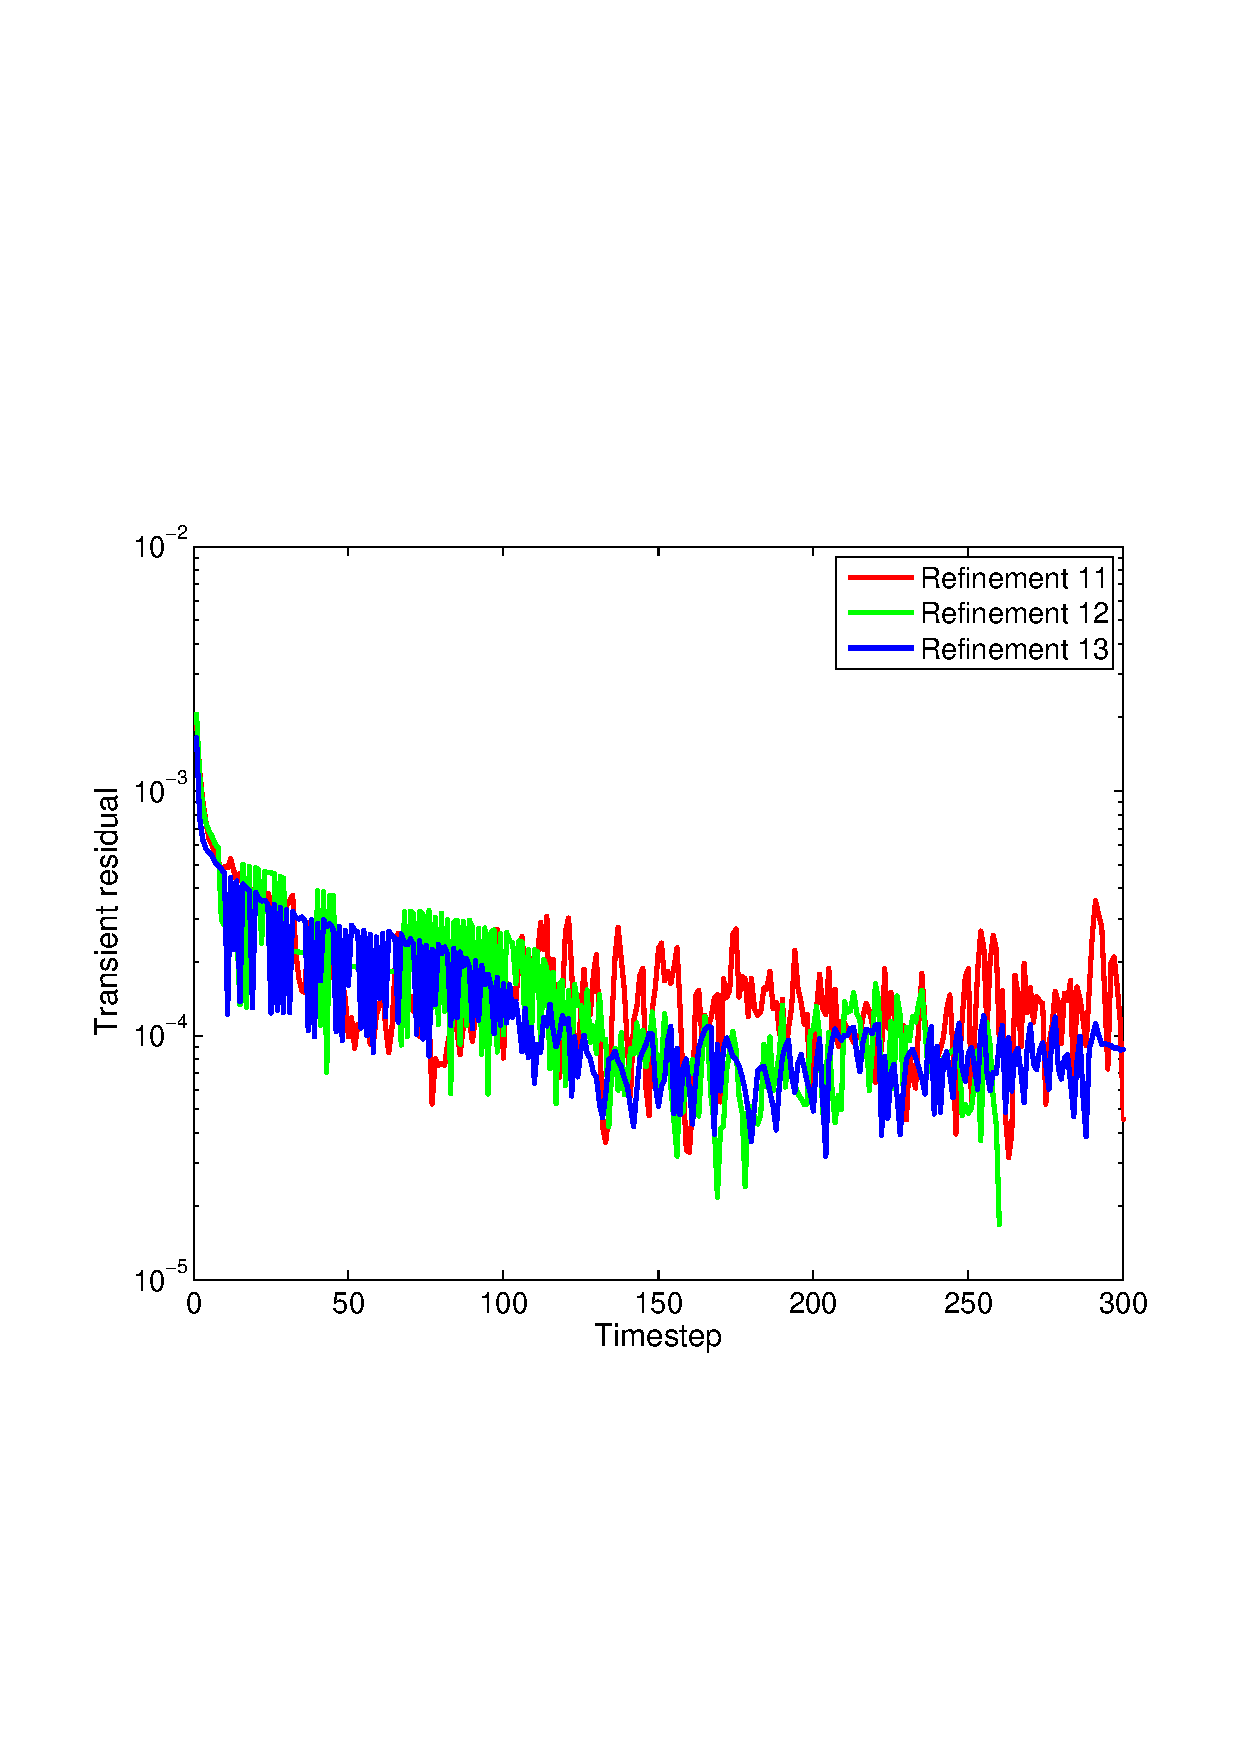
\includegraphics[width=2.5in]{oscillations1.pdf}}
\subfigure[Recovery of convergence]{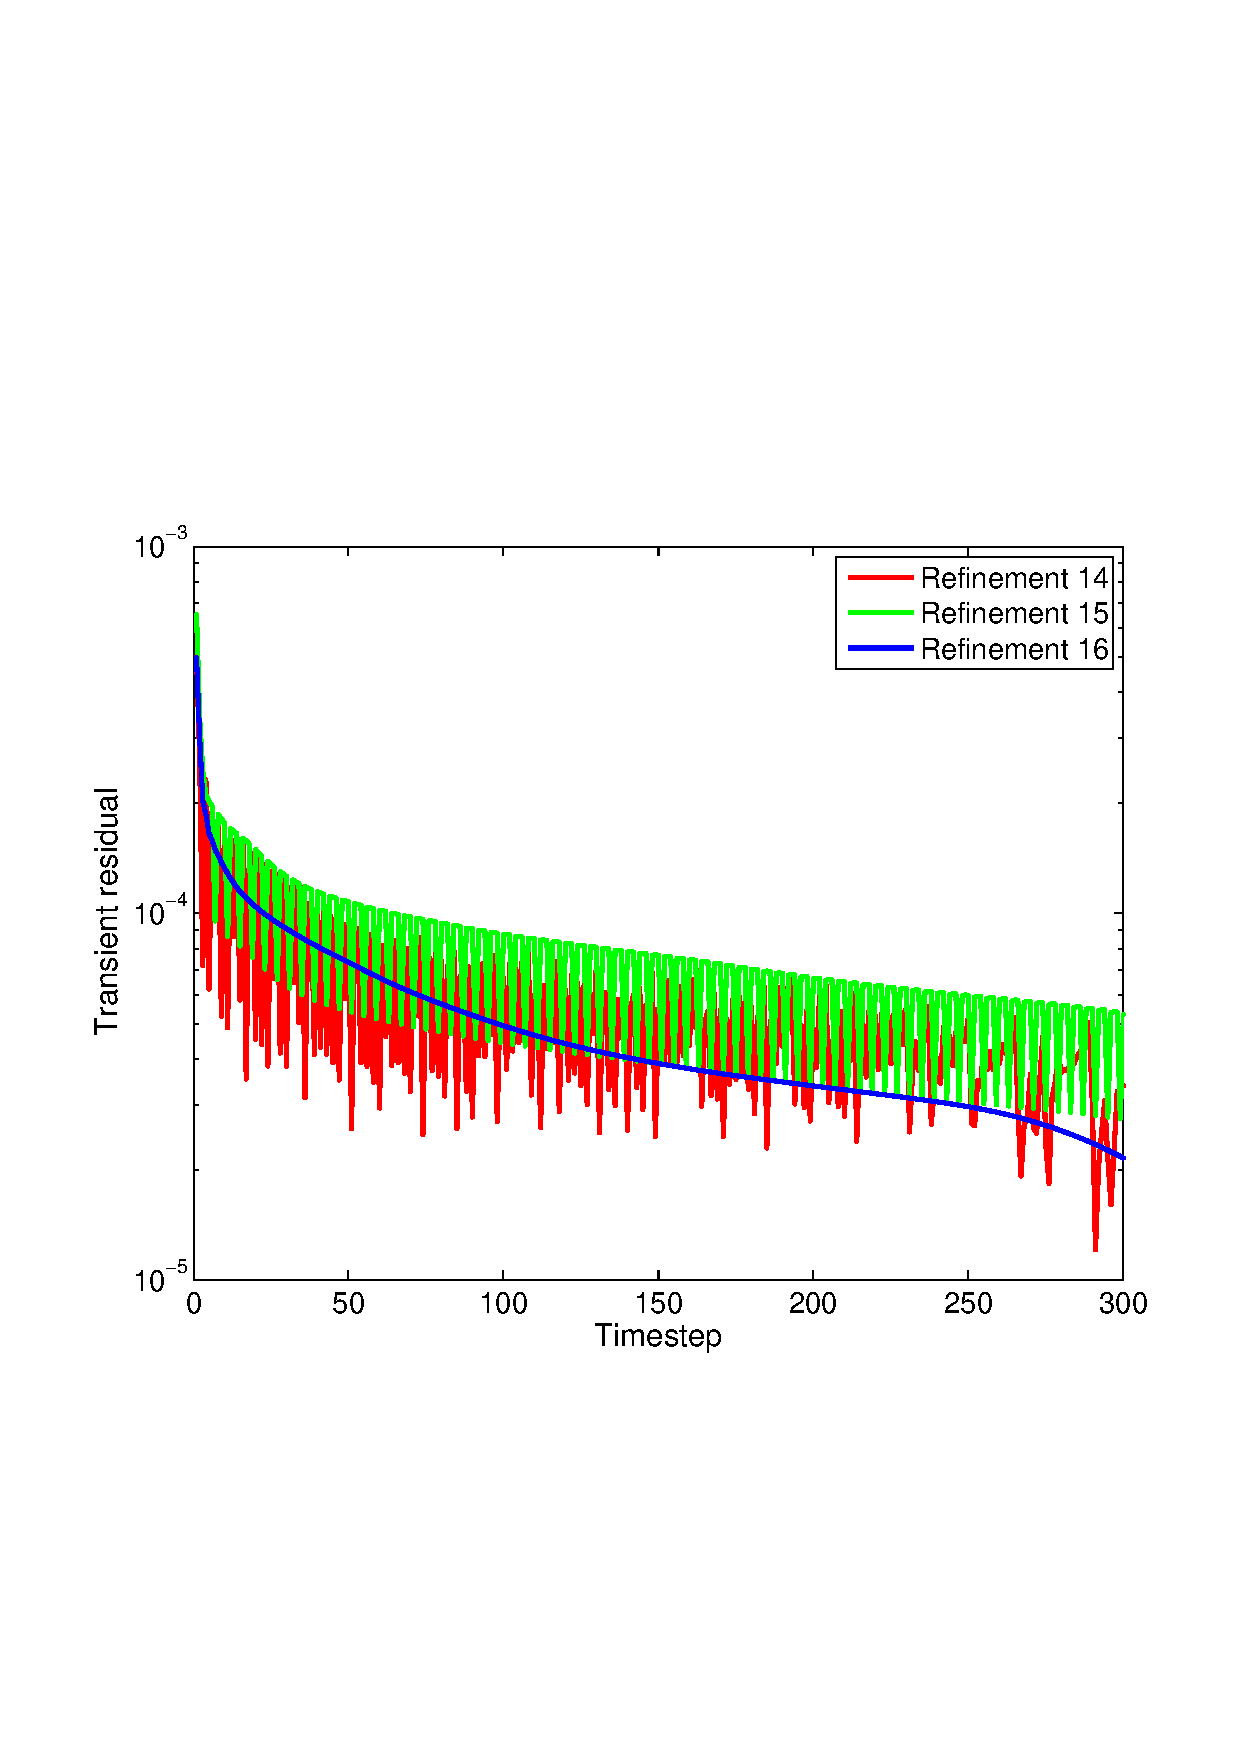
\includegraphics[width=2.5in]{oscillations2.pdf}}
\caption{Stalling and recovery of the pseudo-timestep iteration for $\Reyn = 10000$.}
\label{fig:nonconvergence}
\end{figure}
An examination of the difference in the solutions between the final and $125$th timesteps shows that the nonconvergence of the transient residual is due to oscillations in the solution (primarily in $\rho$) slightly upstream to the plate edge.  Visually, the solution converges everywhere else, save for this area.  Such behavior is also observed in \cite{BenKirk}, where, at the change in boundary conditions between the free stream and flat plate, an oscillation was observed in the solution which prevented convergence of his pseudo-time algorithm.  His oscillations are of smaller magnitude ($O\LRp{10^{-6}}$ as opposed to $O\LRp{10^{-4}}$), which may be the result of several differences between the methods presented.\footnote{Apart from the use of a standard Galerkin (continuous as opposed to discontinuous Galerkin) formulation, Kirk's approach differed from ours in the use of linear elements and the addition of artificial diffusion shock-capturing terms, both of which could explain the lower point at which error stagnates. Reasons for this loss of convergence in the pre-asymptotic range should be explored further.}  However, we note that, under additional refinements and increased resolution of the solution, the transient residual once again decreases in a smooth monotonic fashion, as shown in Figure~\ref{fig:nonconvergence}. 

\begin{figure}
\centering
\subfigure[$\rho$]{\includegraphics[width=2.8in]{rhoRe4Plate.png}}
\subfigure[$u_1$]{\includegraphics[width=2.8in]{u1Re4Plate.png}}
\subfigure[$u_2$]{\includegraphics[width=2.8in]{u2Re4Plate.png}}
\subfigure[$T$]{\includegraphics[width=2.8in]{TRe4Plate.png}}
\caption{Solutions after 18 refinements for $p=2$ and $\Reyn = 10000$.}
\label{fig:Re10000}
\end{figure}

For additional computational efficiency, we also implemented an anisotropic refinement scheme.  In 2D, the boundary layer is a primarily 1D phenomena, which we expect to be far better resolved by anisotropic refinement than by isotropic refinement.  We experimented first using the scheme described in Section~\secref{sec:aniso} as an anisotropy indicator; however, the anisotropic scheme appeared to be too conservative near the boundary layer, placing primarily isotropic refinements.  We modified our scheme in two ways -- first, we incorporated spatially variable thresholding.  Typically, anisotropic refinement in the $x$ direction is chosen if $e_{x,K} > \epsilon_r e_{y,K}$ (and vice versa for anisotropic refinement in the $y$-direction), where $e_{x_i,K}$ is the error in the $x_i$ direction.  We set $\epsilon_r = \epsilon_{r,K}$; in other words, we allow our anisotropic threshold to vary element-by-element, and decrease it from $\epsilon_r= 10$ to $\epsilon_{r,K} = 2.5$ for elements adjacent to the wall upon which the boundary layer forms.  Additionally, since the boundary layer typically displays rapid variation in the $y$-direction (the direction orthogonal to the wall), we relax the condition under which a vertically cut anisotropic refinement occurs to
\[
2 e_{y,K} > \epsilon_{r,K} e_{x,K}.
\]
Despite the artificial modification of the anisotropic refinement scheme, the resulting meshes still resolve boundary layer solutions more efficiently than isotropic refinements.  We hope to investigate reasons for the ineffectiveness of the pure anisotropic scheme for the compressible Navier-Stokes equations in future research.  

\begin{figure}
\centering
\subfigure[$\rho$]{\includegraphics[width=2.8in]{rhoRescaledRe4Plate.png}}
\subfigure[Mesh]{\includegraphics[width=2.8in]{meshRe4Plate.png}}
\caption{Rescaled solution for $\rho$ in the range $[\rho_{\min},2]$ and adapted mesh.}
\label{fig:rhoScaled}
\end{figure}

\begin{figure}
\centering
\subfigure[$\rho$]{\includegraphics[width=2.8in]{rhoZoomRe4Plate.png}}
\subfigure[$u_1$]{\includegraphics[width=2.8in]{u1ZoomRe4Plate.png}}
\subfigure[$u_2$]{\includegraphics[width=2.8in]{u2ZoomRe4Plate.png}}
\subfigure[$T$]{\includegraphics[width=2.8in]{TZoomRe4Plate.png}}
\caption{Zoom of solutions at the beginning of the plate for $p=2$ and $\Reyn = 10000$.}
\label{fig:Re1e4Zoom}
\end{figure}

We note that the resolution of the solution near the plate edge in Figure~\ref{fig:Re1e4Zoom} for Reynolds number 10000 is qualitatively rougher than that for Reynolds 1000 in Figure~\ref{fig:Re1000_zoom}; this is due to the greedy refinement algorithm emphasizing refinements most strongly at the singular point and not in shock resolution, as well as the fact that at a higher Reynolds number, the shock width is thinner and more difficult to resolve.  Further refinement steps improve resolution of the shock features.  

%\begin{figure}[!h]
%\centering
%\subfigure[${\rm Re} = 1000$]{\includegraphics[scale=.5]{figs/Re1000p2/heatflux.png}}
%\subfigure[${\rm Re} = 10000$]{\includegraphics[scale=.3]{figs/Re1e5/q2line.png}}
%\caption{Heat flux at the bottom boundary.}
%\end{figure}

\subsection{Holden ramp problem}

Our second problem is a modified version of the Holden ramp problem, which models supersonic/hypersonic flow over a compression corner (the geometry of which is given in Figure~\ref{fig:holdenCartoon}).  Similarly to the Carter flat plate problem, a flat plate disrupts the flow and forms a weak shock at the plate tip due to viscous effects and no-slip boundary conditions.  The boundary layer grows down the plate edge, deflecting upwards due to the presence of the compression corner.  A stronger shock forms slightly upstream of the compression corner in order to deflect the incoming supersonic flow, and is a common test problem for adaptive finite element methods for compressible flow \cite{Rachowicz1997231,Barter,BenKirk}.  

\begin{figure}
\centering
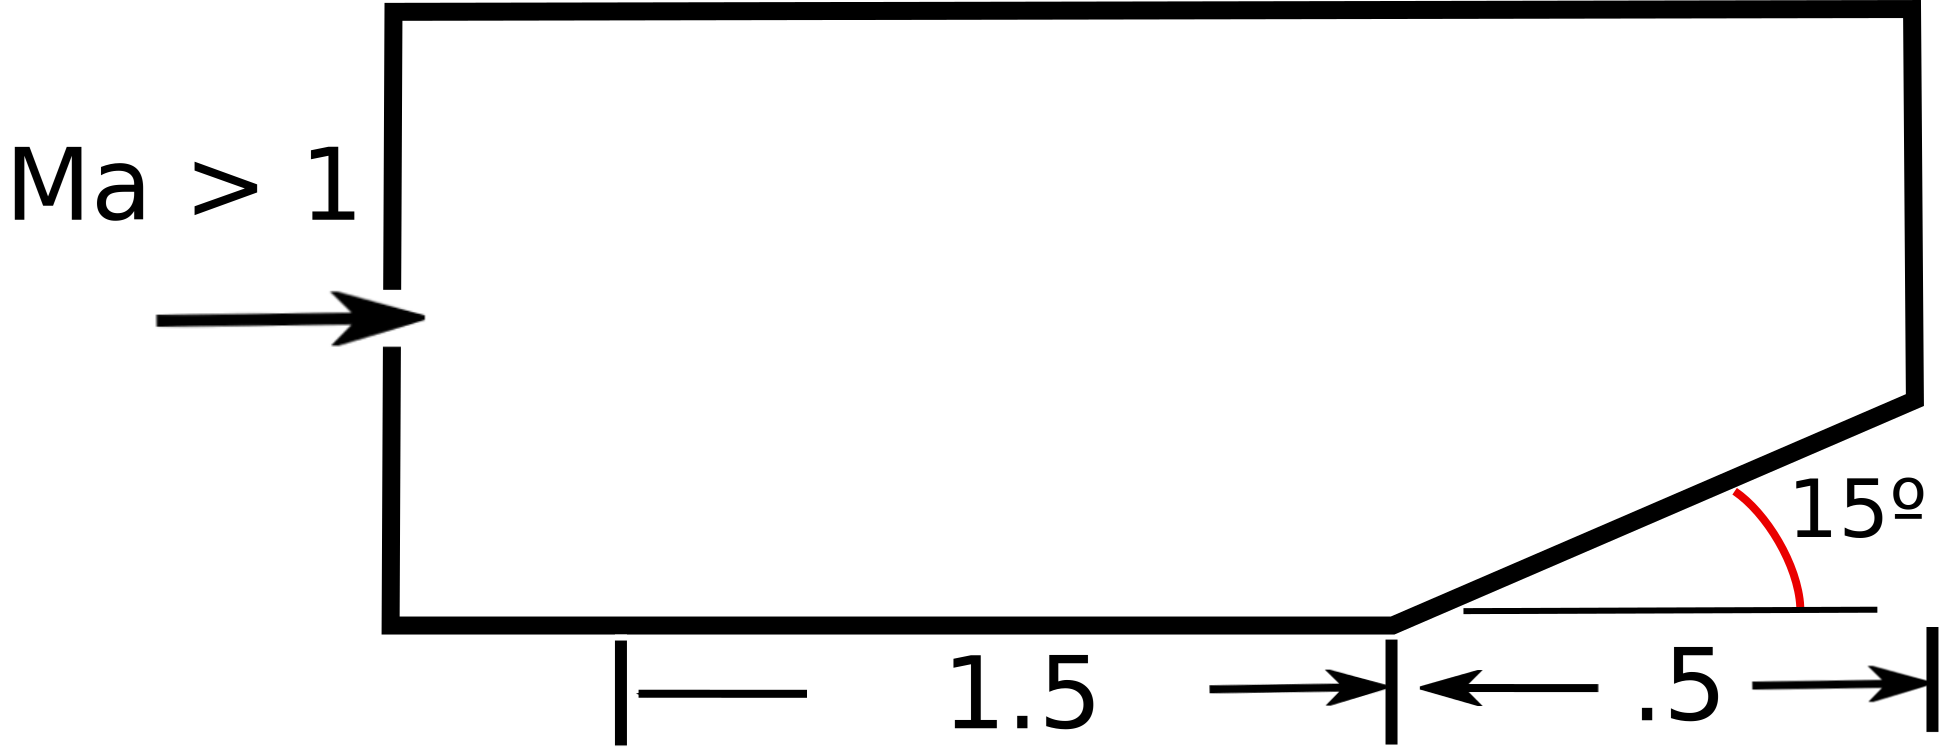
\includegraphics[width=4in]{holden.pdf}
\caption{A modification of the Holden ramp/compression corner problem.}
\label{fig:holdenCartoon}
\end{figure}

The original plate length is given to be .442, while the ramp length is given to be .269. We have modified the problem slightly in order to exactly represent the boundary conditions on a coarse mesh while keeping the ratio of plate length to ramp length roughly the same. Similarly to the Carter flat plate, we start out with a very coarse $2 \times 3$ mesh of 6 elements.  We initialize our solution to the freestream values
\[
\rho_{\infty} = 1,\qquad u_{1,\infty}= 1,\qquad u_{2,\infty} = 0, \qquad T_{\infty} = 1
\]
and again set stresses uniformly to zero.   

\begin{figure}
\centering
\subfigure[$\rho$ rescaled]{\includegraphics[width = 2.9in]{rhoRescaledMa6Ramp.png}}
\subfigure[$u_1$]{\includegraphics[width = 2.9in]{u1Ma6Ramp.png}}
\subfigure[$u_2$]{\includegraphics[width = 2.9in]{u2Ma6Ramp.png}}
\subfigure[$T$]{\includegraphics[width = 2.9in]{TMa6Ramp.png}}
\subfigure[Mesh]{\includegraphics[width = 5.5in]{meshMa6Ramp.png}}
\caption{Solutions and adaptive mesh for ${\rm Ma} = 6$ and $\Reyn = 10000$.}
\label{fig:holdenMa6}
\end{figure}

We first solve under Mach 6 flow.\footnote{The increase in Mach number is to change the angle of the shock; under the current setup, Mach 3 flow produced a shock which reflected off the top boundary $y = 1$  We note that the effect of Mach number under our nondimensionalization of choice is to decrease the thermal diffusivity constant $\kappa$ relative to the viscosities $\mu$ and $\lambda$.} and Reynolds number of 10,000, or a Reynolds number of 33,936 if measured with respect to the original plate length of .442.  The wall temperature is set to $T_{w} = 2.8T_{\infty}$, identically to the flat plate problem.  24 mesh refinements were performed, resulting in a final mesh of 1858 elements.  Figure~\ref{fig:holdenMa6} shows both solution values and final adaptive mesh.  Due to a large maximum value of $\rho_{\max} = 14.1538$ at the plate tip, the resulting solution for $\rho$ is scaled to better show qualitative features of the flow.  The presence of the second shock deflecting the incoming supersonic flow at the ramp is clearly seen in both the solutions and the adaptive mesh refinements.  

\begin{figure}
\centering
\subfigure[Initial mesh]{\includegraphics[width = 2.9in]{rampMesh0.png}}
\subfigure[6 refinements]{\includegraphics[width = 2.9in]{rampMesh6.png}}
\subfigure[12 refinements]{\includegraphics[width = 2.9in]{rampMesh12.png}}
\subfigure[18 refinements]{\includegraphics[width = 2.9in]{rampMesh18.png}}
\caption{Sequence of adaptive meshes for ${\rm Ma} = 6$ and $\Reyn = 10000$.}
\label{fig:holdenMa6Meshes}
\end{figure}

We can examine the sequence of adaptive meshes generated by the DPG method.  Figure~\ref{fig:holdenMa6Meshes} shows the initial mesh, as well as the 6th, 12th, and 18th subsequent refinements generated automatically by the DPG method.  Unlike the previous sequence of meshes generated by the flat plate example, refinements tend to be placed most heavily near the shock at the outflow ramp.  By the 18th refinement, the adaptive mesh looks qualitatively very similar to the final mesh of 24 refinements, and further refinements focus on the resolution of the shocks originating at the plate edge and at the ramp outflow.  

\begin{figure}
\centering
\subfigure[$\rho$ rescaled]{\includegraphics[width = 2.9in]{rhoRescaledshockMa6Ramp.png}}
\subfigure[$T$]{\includegraphics[width = 2.9in]{TshockMa6Ramp.png}}
\subfigure[Mesh]{\includegraphics[width = 4in]{shockMeshMa6Ramp.png}}
\caption{Zoom of solutions and adaptive mesh around shock. }
\label{fig:holdenMa6Zoom}
\end{figure}

Figure~\ref{fig:holdenMa6Zoom} shows a zoom of the second stronger shock that develops near the ramp outflow.  Refinements are placed very heavily near the shock, which we expect due to the fact that a shock forms a stronger gradient than a boundary layer.  We note that our residual-driven adaptivity scheme places mesh refinements in a very precise manner; refinements on ramp boundary are placed slightly more heavily upstream than downstream.  We believe this is due to the fact that solution gradients are slightly higher in $\rho$ at the upstream section of the ramp.  

\begin{figure}
\centering
\subfigure[$\rho$ rescaled]{\includegraphics[width = 2.9in]{rhoRescaledMa11Ramp.png}}
\subfigure[$u_1$]{\includegraphics[width = 2.9in]{u1Ma11Ramp.png}}
\subfigure[$u_2$]{\includegraphics[width = 2.9in]{u2Ma11Ramp.png}}
\subfigure[$T$]{\includegraphics[width = 2.9in]{TMa11Ramp.png}}
\subfigure[Mesh]{\includegraphics[width = 5.5in]{meshMa11Ramp.png}}
\caption{Solutions and adaptive mesh for ${\rm Ma} = 11.68$ and $\Reyn = 16442.4$.}
\label{fig:holdenMa11}
\end{figure}

The second set of conditions under which we solve are under Mach 11.68 flow and Reynolds number of 16,4	42.4, or 55,800 if measured with respect to original plate length, with the wall temperature set to $T_{w} = 4.6T_{\infty}$.  24 automatic mesh refinements are performed under an energy threshold of $.5$, resulting in a final mesh of 2385 elements.  

Figure~\ref{fig:holdenMa11} shows the resulting solution and final adaptive mesh.  The increased Mach number changes again the angle of the weak shock resulting from the change in boundary conditions at the plate edge.  Compared to the previous case of Mach 6 flow, where only 18 refinements steps were performed, 24 refinements were performed for the Mach 11.68 case, leading to a more highly resolved solution, especially near the plate tip.  Due to a large maximum value of $\rho_{\max} = 50.1805$ at the plate tip, the resulting solution for $\rho$ is scaled to better show qualitative features of the flow.  

%We note that, under a higher Mach number, the placement of adaptive mesh refinements appears to improve.  The element size adjacent to the plate tip for the Mach $6$ case is $h = O\LRp{10^{-4}}$, while the size of elements adjacent to the plate tip in the Mach 11 case is $h = O\LRp{10^{-5}}$.  For the Mach $6$ and Reynolds $10,000$ case of the ramp problem, several extraneous refinements were placed slightly upstream of the plate tip, corresponding to the location of large gradients in the Newton solution update.  More study is necessary to determine the reasons for the difference in behavior of the automatic adaptivity algorithm.
%
%\begin{figure}[!h]
%\centering
%%\subfigure[$\rho$]{\includegraphics[width = 2.9in]{rhoshock.png}}
%%\subfigure[$T$]{\includegraphics[width = 2.9in]{Tshock.png}}
%\subfigure[Mach 6]{\includegraphics[width = 2.75in]{plateMesh.png}}
%\subfigure[Mach 11]{\includegraphics[width = 2.75in]{plateMesh.png}}
%\caption{Zoom of solutions and adaptive mesh around the plate tip.}
%\label{fig:plateComparison}
%\end{figure}

\begin{figure}
\centering
\subfigure[$\rho$ rescaled]{\includegraphics[width = 2.9in]{rhoshockMa11Ramp.png}}
\subfigure[$T$]{\includegraphics[width = 2.9in]{TshockMa11Ramp.png}}
\subfigure[Mesh]{\includegraphics[width = 4in]{shockMeshMa11Ramp.png}}
\caption{Zoom of solutions and adaptive mesh around shock. }
\label{fig:holdenMa11Zoom}
\end{figure}

Compared to the Mach 6 case, where 18 refinements were performed, the resolution of the mesh near the shock at the ramp outflow for Mach 11.68 flow and 18 refinements is qualitatively similar.  Further refinement steps increase resolution of the mesh near the shock, as shown in Figure~\ref{fig:holdenMa11Zoom}.  

Finally, we plot the normal heat flux over the plate and ramp for both Holden problems in Figure~\ref{fig:heatFlux}.  The normal heat flux over the flat plate is indicated by the blue line, while the dotted brown line indicates the heat flux over the ramp, and both are plotted against the x-coordinate along the plate/ramp boundary.  The normal heat flux is given by the normal trace of the conserved quantity in the energy equation
\[
\widehat{f}_{4,n} = (\rho e+p)u_n - \boldsymbol n\cdot \boldsymbol \sigma\cdot \boldsymbol u + q_n.
\]
Recognizing that $u_1 = u_2 = 0$ reduces the above to $\widehat{f}_{4,n} = q_n$.  

The heat flux develops a strong singularity at the point $(-.5,0)$, where the boundary condition changes from a Neumann/stress boundary condition to a Dirichlet/no-slip boundary condition.\footnote{Figure~\ref{fig:heatFlux} cuts off this singularity in order to show the qualitative behavior of $q_n$ over the remainder of the boundary.  The maximum visualized values in the singular portion of $q_n$ are .35 for Mach 6 flow and 1.268 for Mach 11.68 flow.}  It can be shown that the Laplace equation develops a singularity in stress at under any such change in boundary conditions, and the same phenomena is observed for a similar setup under convection-diffusion \cite{localConservationDPG}.  

\begin{figure}
\centering
\subfigure[Mach 6, Reynolds 10,000]{\includegraphics[width=2.9in]{heatFluxMa6Ramp.png}}
\subfigure[Mach 11.68, Reynolds 16,442.4]{\includegraphics[width=2.9in]{heatFluxMa11Ramp.png}}
\caption{Normal heat flux $q_n$ over plate and ramp for the Holden problem.  The blue line indicates $q_n$ over the flat plate, while the brown line indicates $q_n$ over the ramp. }
\label{fig:heatFlux}
\end{figure}

\subsection{Higher Reynolds numbers}
\seclab{sec:oscillations}
For higher Reynolds number, the pseudo-timestepping, we have encountered difficulties which have made it difficult to converge to a steady-state solution, even under the addition of an effective CFL number and line search to enforce positivity of density $\rho$ and temperature $T$.  However, we believe these difficulties to be related to the nature of the equations, rather than the robustness of the method.  We illustrate this with a simple example.  

Let us consider the 1D steady state viscous Burgers' equation on $[-\infty,\infty]$
\[
u\pd{u}{x} - \epsilon \pdd{u}{x} = 0.
\]
The exact solution to this equation under boundary conditions
\begin{align*}
u(-\infty) &= 1\\
u(\infty) &= -1
\end{align*}
can be easily derived (see \cite{Barter} for a simple derivation), and the solution and its first two derivatives are
\[
u(x) = \frac{1-e^{\frac{x}{\epsilon}}}{1+e^\frac{x}{\epsilon}}, \qquad u'(x) = \frac{-2e^{\frac{x}{\epsilon}}}{\LRp{1+e^{\frac{x}{\epsilon}}}^2\epsilon}, \qquad u''(x) = \frac{-2e^{\frac{x}{\epsilon}}\LRp{e^{\frac{x}{\epsilon}}-1}}{\LRp{1+e^{\frac{x}{\epsilon}}}^3\epsilon^2}
\]
\begin{figure}
\centering
\subfigure[$u(x)$]{\includegraphics[width = 1.8in]{u.pdf}}
\subfigure[$u'(x)$]{\includegraphics[width = 1.8in]{du.pdf}}
\subfigure[$u''(x)$]{\includegraphics[width = 1.8in]{ddu.pdf}}
\caption{$u(x)$ and its derivative and second derivative for $\epsilon = .01$.}
\label{fig:burgersSoln100}
\end{figure} 
Figure~\ref{fig:burgersSoln100} shows each of these functions for $\epsilon = .01$.  From the form of $u'(x)$ and $u''(x)$, we know these oscillations will grow rapidly as $\epsilon$ decreases.  Consider now the linearized Burgers' equation
\[
\pd{u\Delta u}{x} - \epsilon \pdd{\Delta u}{x} = - r(x)
\]
where $r(x) = u\pd{u}{x} - \epsilon \pdd{u}{x}$ is the strong form of the nonlinear residual.  Recall that for a pure Newton iteration, $u(x)$ is assumed to be known, and the linearized problem is driven by the residual.  The solution $u(x)$ is updated $u \coloneqq u + \Delta u$, and is repeated until $\Delta u$ and $r(x)$ are both approximately zero.

Let $u_\epsilon(x)$ be the exact solution for a particular viscosity $\epsilon$, and consider the setting of $u(x) = u_{\alpha \epsilon}(x)$, with $\alpha > 1$.  In other words, the initial guess for the Newton iteration is taken to be the exact solution for the viscous Burgers' equation under a larger viscosity (a less sharp shock), a method known as continuation (specifically, continuation in viscosity $\epsilon$).\footnote{We note that continuation in Reynolds number was attempted for the Navier-Stokes equations; however, the presence of large oscillations in the Newton update on highly adapted meshes caused the line search to return a near-zero step length, which stalled the nonlinear iteration prior to convergence to a steady state solution.}

\begin{figure}
\centering
\subfigure[$\epsilon = .01$]{\includegraphics[width = 2.5in]{residual100.pdf}}
\subfigure[$\epsilon = .001$]{\includegraphics[width = 2.5in]{residual1000.pdf}}
\caption{Residual for Burgers' equation with viscosity $\epsilon$ under the exact solution for ${2\epsilon}$.}
\label{fig:burgersResidual}
\end{figure} 

We plot $r(x)$ for $u(x) = u_{2\epsilon}(x)$ in Figure~\ref{fig:burgersResidual}.  While the form of the exact linearized solution $\Delta u$ is unknown, we see that the forcing term in the above equation develops oscillations that grow in magnitude and decrease in support as $\epsilon$ decreases.  We have observed similar behaviors for discretized solutions to the Burgers' and Navier Stokes equations -- the discrete linearized solution will develop gradients as well, though their magnitude will be limited by the resolution of the mesh.  However, additional refinements near shocks will introduce additional oscillations, which are subsequently damped by additional Newton iterations.  

In other words, not all oscillations are related to the method of discretization -- the exact linearized solution itself contains large oscillations, which are picked up more and more strongly in a discrete scheme as the mesh resolution approaches the viscous length scale $\epsilon$ (see \cite{DPGspacetime, DPGNS_1d} for additional numerical examples).  We note that these large oscillations are not an issue for the viscous Burgers' equation, as there is no positivity constraint on $u$.  However, as noted previously, the convergence of the nonlinear iteration for the compressible Navier-Stokes equations can stall or even diverge for sufficiently negative values of $\rho$ and $T$, which happens easily in the presence of large oscillations.  When a line search is implemented to enforce a strictly positive solution, the nonlinear iteration can stall, and numerical experiments have generated cases in which the line search length goes to zero, returning an under-converged solution.  

There are several approaches to controlling the magnitude of oscillations in the linearized solution -- a simple option is decreasing the size of the timestep; however, doing so can cause the number of iterations required for convergence to greatly increase.  The application of artificial diffusion near sharp gradients is another way in which to control such oscillations; however, this results in a modified set of equations, and, though solutions with contemporary artificial viscosity methods can produce solutions with expected qualitative features, there is a wide range of choices for artificial diffusion, and it was not clear in the scope of this paper which artificial viscosity method would be quantifiably superior, or most suitable for use with the DPG method.  



\section{Conclusions and future work}

The goal of this work has been to explore the behavior of the Discontinuous Petrov-Galerkin (DPG) method as a method for the discretization and solution of convection-dominated diffusion problems, and to produce both theory and numerical results for model problems in this area.  We begin by introducing the DPG method for linear problems; the concept of problem-dependent optimal test functions is derived through equivalence with the minimization of a specific residual, and discontinuous test functions are introduced in order to localize the determination of such optimal test functions to a single element.  

The DPG framework is then extended to nonlinear problems, and equivalence is shown between the DPG method and a Gauss-Newton minimization scheme for the nonlinear residual.  An anisotropic refinement scheme is implemented to more effectively capture lower-dimensional behavior of solutions of convection-diffusion problems, such as boundary layers.  We extrapolate the DPG method to a nonlinear viscous Burgers' equation, and conclude by applying the DPG method to systems of equations and to the solution of two model problems in viscous compressible flow.  

In particular, we demonstrate for both the flat plate and compression ramp problem in supersonic/hypersonic in compressible flow that the DPG method is able to begin from a highly underresolved meshes (two elements for the Carter plate problem, and 12 elements for the Holden ramp problem), and resolve physical features of the solution through automatic adaptivity, without the aid of artificial diffusivity or shock capturing terms.  We believe this indicates both the robustness of the method on coarse grids and the effectiveness of the DPG error indicator for adaptive refinement.  

As is the case with any research, much work remains to be done.  We have chosen the classical variables in which to cast the compressible Navier-Stokes equations; however, investigation of alternative sets of variables may have merit, as different choices of variables yield differing linearizations with their own advantages (for example, all derivatives in time are linear with respect to the momentum variables, and the entropy variables of Hughes both symmetrize the Navier-Stokes equations and yield solutions obeying second law of thermodynamics for standard $H^1$ formulations \cite{Hughes1986223}).  

We also hope to investigate artificial viscosity methods as regularization for problems in viscous compressible flow.  We present an analysis of the 1D Burgers' equation demonstrating that the exact solutions under Newton linearization contain large oscillations.  While these oscillations are not the result of the stability of the spatial discretization, their presence can cause density and temperature to become non-physically negative, which can stall the convergence of the nonlinear solver.  Our goal in incorporating artificial viscosity would not be to provide additional stabilization mechanisms for the discrete spatial discretization, but to provide regularization with which to suppress the presence of large oscillations in the linearized solution.  

Finally, though the method is inf-sup stable for arbitrary meshes, our experiments have focused on meshes of uniform $p$.  We hope to implement a true $hp$-adaptive DPG method in the future.  

%\bibliographystyle{plain}
\bibliographystyle{unsrt}
\bibliography{paper,NSNotes,DPGarticles}

\end{document}
